%search for nnnote for things to resolve later.

\RequirePackage[l2tabu, orthodox]{nag}

\documentclass[letterpaper, 12 pt]{report}

\usepackage[T2A, T1]{fontenc}
\usepackage[utf8]{inputenc}
\usepackage{lmodern}
\usepackage{CJKutf8}
\usepackage{amsfonts}
\usepackage{amsmath}
\usepackage{amssymb}
\usepackage{braket}
\usepackage{ellipsis}
\usepackage{microtype}
\usepackage[ocgcolorlinks]{hyperref}
\usepackage[numbers,sort&compress]{natbib}
\usepackage{graphicx}
\usepackage[usenames,dvipsnames]{xcolor}

%change link colours:
\hypersetup{ linktocpage, colorlinks=true, linkcolor=blue,
             citecolor=blue, filecolor=blue, urlcolor=blue }

%Bibliography stuff:
\bibliographystyle{ieeetr}
\usepackage{etoolbox}
\renewcommand\bibname{References}
\apptocmd{\thebibliography}{\raggedright}{}{}

\title{Dissertation: early version}
\author{Matthew Baxter}
\date{\today}

\begin{document}

\pagenumbering{alph}

\begin{titlepage}
   
   \maketitle
   \thispagestyle{empty}

\end{titlepage}

\cleardoublepage
\phantomsection
\addcontentsline{toc}{chapter}{Abstract}

\begin{abstract}
   
   \thispagestyle{plain}
   \pagenumbering{roman}
   \setcounter{page}{2}

\end{abstract}

\setcounter{page}{3}

\cleardoublepage
\phantomsection
\addcontentsline{toc}{chapter}{Contents}
\tableofcontents

\cleardoublepage
\phantomsection
\addcontentsline{toc}{chapter}{List of Tables}
\listoftables

\cleardoublepage
\phantomsection
\addcontentsline{toc}{chapter}{List of Figures}
\listoffigures

\newpage

\pagenumbering{arabic}

\begin{chapter}{Introduction \label{chap:intro}}

\end{chapter}

\begin{chapter}{Density Functional Theory \label{chap:dft}}

   This chapter concerns itself with a brief introduction to the world of density-functional theory,
   both ground-state~\cite{dft-engel} (DFT) and time-dependent~\cite{tddft, marques-1} (TDDFT). This
   discussion begins with a discussion of various existence theorems central to density functional
   theory (Sec.~\ref{sec:dft}). Next the Kohn-Sham equations are introduced in Sec.~\ref{sec:ks}.
   More practical matters are considered when the two main problems of density functional theory,
   the observable problem (Sec.~\ref{sec:obs}) and the determination of the exchange-correlation
   potential (Sec.~\ref{sec:xcpot}) are introduced. The discussion of the xc-potential is focused on
   the optimized potential method (Sec.~\ref{sec:opm}) and the Krieger-Li-Iafrate approximation
   (Sec.~\ref{sec:kli}).

   \begin{section}{DFT and TDDFT Existence Theorems \label{sec:dft}}

      In the standard treatment of many-body quantum mechanics a system is described by a wavefunction
      $\Psi$ which, depending upon the situation, is determined by either time-dependent Sch\"{o}dinger
      equation (TDSE)
      %
      \begin{equation} \label{eq:tdse}
         \hat{H}(t) \Psi(t) = i \frac{\mathrm{d} \Psi(t)}{\mathrm{d} t},
      \end{equation}
      %
      or the stationary Sch\"{o}dinger equation (SSE)
      %
      \begin{equation} \label{eq:sse}
         \hat{H} \Psi = E \Psi.
      \end{equation}
      %
      If the system in question consists of $N$ non-relativistic electrons then $\Psi$ becomes a
      function $N$ position variables $\mathbf{r}_i$ and spin variables $\sigma_i$. The Hamiltonian,
      $\hat{H}$, may be decomposed into a kinetic energy term
      %
      \begin{equation} \label{eq:Top} %nnnote: tfrac or normal frac?
         \hat{T} = -\frac{1}{2} \sum\limits^{N}_{i=1} \Delta_i,
      \end{equation}
      %
      an electron-electron term
      %
      \begin{equation} \label{eq:Vee} %nnnote: tfrac or normal frac?
         \hat{V}_{ee} = \frac{1}{2} \sum\limits^{N}_{i \neq j}
                        \frac{1}{\left| \mathbf{r}_i - \mathbf{r}_j \right|},
      \end{equation}
      %
      and a, possibly, time-dependent external potential
      %
      \begin{equation} \label{eq:Vext}
         \hat{V}_\mathrm{ext} = \sum\limits^{n}_{i = 1} v_\mathrm{ext} (\mathbf{r}_i, \sigma_i, t).
      \end{equation}
      %
      The function $\hat{V}_\mathrm{ext}$ contains all of the one-body interactions, including the
      nuclear and any external potentials.

      Given the one-particle electronic density
      %
      \begin{equation} \label{eq:dendef1}
         n(\mathbf{r}, t) = N \sum\limits_{\sigma_i} \int \mathrm{d}^3 r_2 \dots \mathrm{d}^3 r_N
                            \left| \Psi(\mathbf{r}, \sigma_1, \mathbf{r}_2, \sigma_2, \dots,
                                   \mathbf{r}_N, \sigma_N) \right|^2
      \end{equation}
      %
      the Hohenberg–Kohn theorem~\cite{hk-theorem} in the stationary case and the Runge-Gross
      theorem~\cite{rgt} in the time-dependent case establish a one-to-one mapping between the
      one-particle density $n$ and the external potential $\hat{V}_\mathrm{ext}$. The potential is
      then a unique functional of the one-particle density
      %
      \begin{equation} \label{eq:vext-func}
         \hat{V}_\mathrm{ext} = \hat{V}_\mathrm{ext} [n].
      \end{equation}
      %
      It should be noted that for time-dependent systems this mapping is unique only up to the addition
      of an arbitrary time-dependent function, as this serves only to introduce a phase into the
      associated wave function $\Psi[\hat{V}_\mathrm{ext}]$ it can be safely ignored in all future
      discussions.

      We have formulated the density-potential mapping for an explicitly spin-dependent system, it
      then be noted that the original existence theorems we not formulated in such general terms.
      Luckily, generalizations for both the stationary~\cite{spin-dep1, spin-dep2} and
      time-dependent~\cite{td-spindep} to spin-polarized systems exist.

   \end{section}

   \begin{section}{The Kohn-Sham Equations \label{sec:ks}}

      In practice the correspondence between the density and potential is used to map the interacting
      many-body SSE or TDSE onto an auxiliary non-interacting system. The density-potential mappings
      discussed in the previous section allow one to rewrite the interacting system in terms of
      an auxiliary system of non-interacting particles by the functions $\varphi_{i\sigma}$ ($i = 1,
      \dots, N$) with
      %
      \begin{equation} \label{eq:dendef2}
         n = \sum\limits_{\sigma} \sum\limits_{i = 1}^N
                           \left| \varphi_{i\sigma} \right|^2,
      \end{equation}
      %
      where $n$ is the one-particle density of the fully interacting system. The orbitals $\phi_i$ are
      determined through the stationary or time-dependent Kohn-Sham equations~\cite{ks-eq, spin-dep1,
      spin-dep3} (SKS, TDKS respectively)
      %
      \begin{equation} \label{eq:sks}
         \left( -\frac{\Delta}{2} + v^\sigma_\mathrm{KS}[n_\uparrow, n_\downarrow](\mathbf{r}) \right)
          \varphi_{i\sigma}(\mathbf{r}) = \epsilon_i \varphi_{i \sigma}(\mathbf{r}),
      \end{equation}
      %
      \begin{equation} \label{eq:tdks}
         i \frac{\partial}{\partial t} \varphi_{i\sigma} = 
            \left( -\frac{\Delta}{2} + v^\sigma_\mathrm{KS}[n_\uparrow, n_\downarrow](\mathbf{r},t)
            \right) \varphi_{i\sigma}(\mathbf{r},t),
      \end{equation}
      %
      where the $\epsilon_i$ appearing in Eq.~\eqref{eq:sks} are the Kohn-Sham eigenvalues and the
      quantities $n_\uparrow$, $n_\downarrow$ are the spin-up/down one-particle densities defined by
      %
      \begin{equation} \label{eq:spinden}
         n_\sigma = \sum\limits_{i=1}^{N} \left| \phi_{i\sigma} \right|^2.
      \end{equation}

      The potential in Eqs.~\eqref{eq:sks} and \eqref{eq:tdks} is know as the Kohn-Sham potential. This
      potential may be simplified by splitting it into a series of less complex objects
      %
      \begin{equation} \label{eq:vks}
         v^\sigma_\mathrm{KS}[n_\uparrow, n_\downarrow] = v_\mathrm{ext} + v_\mathrm{H}[n]
            + v_\mathrm{xc}[n_\uparrow, n_\downarrow].
      \end{equation}
      %
      The first term in this expression is the external potential, which is essentially the same as the
      potential $\hat{V}_\mathrm{ext}$ of Eqs.~\eqref{eq:sse} and~\eqref{eq:tdse}. The next term is
      the Hartree screening potential
      %
      \begin{equation} \label{eq:vh}
         v_\mathrm{H}(\mathbf{r},t) = \int \frac{n(\mathbf{r}^\prime, t)}
            {\left| \mathbf{r} - \mathbf{r}^\prime\right|} \, \mathrm{d}^3 r^\prime.
      \end{equation}
      %
      The last term is the exchange-correlation potential which encodes the complicated
      electron-electron interaction potential into the language of the non-interacting system. For
      convenience this is often further broken down into separate exchange and correlation potentials
      %
      \begin{equation} \label{eq:vxc}
         v_\mathrm{xc} = v_\mathrm{x} + v_\mathrm{c}.
      \end{equation}

   \end{section}

   \begin{section}{Observables \label{sec:obs}}

      In the standard treatment of many body quantum mechanics there is a well established process for
      calculating observables from the full many body wave function describing the system. For any
      solution $\Psi$, unique up to a phase factor, of the SSE or TDSE and any observable $\hat{O}$ we
      immediately have the unique functional
      %
      \begin{equation} \label{eq:obsfunc1}
         O[\Psi] = \braket{\Psi| \hat{O} | \Psi},
      \end{equation}
      %
      so long as $\hat{O}$ contains no time derivative terms.

      The density-potential mappings of Sec.~\ref{sec:dft} provide the relation
      %
      \begin{equation} \label{eq:denpot}
         n \mapsto \hat{V}_\mathrm{ext}[n] + c(t).
      \end{equation}
      %
      As the function $c$ only serves to introduce another phase factor we may use the uniqueness of
      solutions of the SSE/TDSE to define a map
      %
      \begin{equation} \label{eq:obsfunc2}
         n \mapsto \hat{V}_\mathrm{ext} \mapsto \Psi \mapsto O
      \end{equation}
      %
      or, $O = O[n]$; the observable is a functional of the one-particle density.

      In principle all observables are functionals of the one-particle density. However, in practice the
      exact functional is only known in a handful of cases~\cite[p. 211-213]{obs_exac}.

   \end{section}

   \begin{section}{xc-potential \label{sec:xcpot}}

      Consider the energy functional for the interacting system
      %
      \begin{equation} \label{eq:efunc}
         E[n] = \braket{\Psi[n] | \hat{H} | \Psi[n] }= T[n] + E_{ee}[n] + E_\mathrm{ext}[n]
      \end{equation}
      %
      where the energies on the right hand side are the contributes from the constituent operators
      Eq.~\eqref{eq:Top}-\eqref{eq:Vext}. Similarly, we may define the energy functional for the
      non-interacting, KS, system as
      %
      \begin{equation} \label{eq:esfunc}
         E_s[n] =  T_s[n] + E_\mathrm{xc}[n] + E_\mathrm{H}[n] + E_\mathrm{ext}[n].
      \end{equation}
      %
      Making use of the fact that the energy is a unique functional of the density it follows that
      %
      \begin{equation} \label{eq:exc}
         E_\mathrm{xc} = T - T_s + E_{ee} - E_\mathrm{H}.
      \end{equation}
      %
      Finally making use of the fact that the ground-state one-particle density will minimize the action
      it follows that
      %
      \begin{equation} \label{eq:vxc-der}
         \frac{\delta E_\mathrm{xc}[n]}{\delta n(\mathbf{r})} = v_\mathrm{xc}[n](\mathbf{r}).
      \end{equation}
      %
      The universality of the xc-functional~\cite{dft-engel} means that once an approximation to
      $E_\mathrm{xc}$ has been found we may apply the resulting potential to any system. Of course,
      some approximations will be better suited to certain situations.

      There are a few caveats to apply Eq.~\eqref{eq:vxc-der}. First, the functional in only defined
      for the set of ground-state $v$-representable densities, those densities which arise as solutions
      of the SSE for some potential $v$. The second problem follows from the first, due to the fact
      that not all densities are $v$-representable~\cite{not-vrep1, not-vrep2, not-vrep3}. For densities
      defined on a lattice~\cite{vrep-lat} as well as the general case~\cite{nonint1, nonint2,
      vrep-levy1, vrep-levy2, vrep-lieb, vrep-rev} both the issue of $v$-representability and the
      existence of the functional derivatives of the energy functional have been addressed.

      In the case of TDDFT one can no longer rely upon minimizing the energy functional when seeking
      solutions. Instead one looks for stationary points of the quantum mechanical
      action~\cite{qmaction} 
      %
      \begin{equation} \label{eq:qmact}
         A[n] = \int^{t_f}_{t_i} \mathrm{d}t
            \braket{\Psi[n] |i\frac{\partial}{\partial t} -\hat{H}(t) | \Psi[n]}.
      \end{equation}
      %
      In analogy to the ground state case the exchange correlation part of the action may be defined in
      terms of the difference between the actions for the interacting and non-interacting systems. We
      then find at a stationary point that
      %
      \begin{equation} \label{eq:tdvxc-der}
         \frac{\delta A_\mathrm{xc}[n]}{\delta n_\sigma(\mathbf{r},t)}
            = v^\sigma_\mathrm{xc}[n](\mathbf{r},t).
      \end{equation}

      In addition to similar issues of $v$-representability and functional differentiability the action
      Eq.~\eqref{eq:qmact} does not distinguish the direction of time and thus its naive use may lead
      to violations of causality~\cite{tddft-causality}. The existence of functional derivatives has
      been established in a similar style as in the stationary case~\cite{td-welldef}. The problem of
      which densities are $v$-representable has also been solve~\cite{td-vrep}. The causality problem
      may be solve in several ways including extending the time domain to the Keldysh
      contour~\cite{caus-sol1} and relaxing the boundary condition on one end point of the time
      interval~\cite{caus-sol2}.

      The simplest explicit density functional is the local density approximation~\cite{ks-eq}. Taking
      things further one is led to the hierarchy of increasingly complex generalized gradient
      approximations and hybrid functionals~\cite{gga+}. For time-dependent systems one may simply apply
      one of the many DFT functionals to arrive at an adiabatic approximation. Going beyond the
      adiabatic approximation is possible, however such functionals are much more complex. As an example
      the fully time-dependent version of the LDA, the local deformation approximation~\cite{TDLDefA1,
      TDLDefA2} (TDLDefA).

      \begin{subsection}{Optimized Potential Method \label{sec:opm}}

         An alternate approach to the explicit density functionals mentioned above is to employ an
         implicit density functional. Then the xc-potential may be determined in directly from the
         KS-orbitals, and their eigenvalues, through a procedure known as the optimized potential
         method~\cite{opm1, opm2} (OPM) for which there are several derivations~\cite{opm1, opm2, opm3,
         opm4, opm5, opm-rev}.

         Without getting reproducing too many long equations one may use Eq.~\eqref{eq:vxc-der} and
         several applications of the chain rule for functional derivatives
         %
         \begin{equation} \label{eq:opm1}
            \begin{split}
               v^\sigma_\mathrm{xc} & = \int \mathrm{d}^3 r^\prime
                  \frac{\delta v^\sigma_\mathrm{KS}(\mathbf{r^\prime})}{\delta n_\sigma(\mathbf{r}) } \\
                                    & \times \sum\limits_{j} \int \mathrm{d}^3 r^{\prime\prime}
               \left\{ \left[ 
               \frac{\delta E_\mathrm{xc}}{\delta \varphi_{j\sigma}(\mathbf{r^{\prime\prime}}) }
               \frac{\delta \varphi_{j\sigma}(\mathbf{r^{\prime\prime}}) }
                    {\delta v^\sigma_\mathrm{KS}(\mathbf{r^{\prime}}) }
               + c.c.
            \right]
            + \frac{\delta \epsilon_k}{\delta v^\sigma_\mathrm{KS}(\mathbf{r^{\prime}})}
              \frac{\partial E_\mathrm{xc}}{\partial \epsilon_k}
            \right\}
            \end{split}
         \end{equation}
         %
         from which the OPM integral equation is then derived. A similar derivation for the
         time-dependent case leads to the time-dependent OPM equation~\cite{tdopm}. In either situation
         an appropriate choice of $E_\mathrm{xc}$ or $A_\mathrm{xc}$ can include both exchange and
         effects~\cite{opm5, tdopm}. With that said the OPM is typically used to calculate exact
         exchange using the functional
         %
         \begin{equation} \label{eq:xfunc}
            \begin{split}
               A_\mathrm{x}[\varphi_{i\sigma}(\mathbf{r},t)]
                 = & E_\mathrm{x}[\varphi_{i\sigma}(\mathbf{r})] \\
                = & -\frac{1}{2} \sum\limits_\sigma \sum\limits_{j,k}
                    \int\mathrm{d}^3 r \mathrm{d}^3 r^\prime
                    \frac{ \varphi^*_{j\sigma}(\mathbf{r},t) \varphi^*_{k\sigma}(\mathbf{r}^\prime,t)
                   \varphi_{j\sigma}(\mathbf{r}^\prime,t) \varphi_{k\sigma}(\mathbf{r},t)}
                   {\left| \mathbf{r} -\mathbf{r}^\prime \right|}.
            \end{split}
         \end{equation}

      \end{subsection}

      \begin{subsection}{KLI \label{sec:kli}}

         The solution of the full OPM integral equation can be quite difficult. To aid in this process
         the Krieger-Li-Iafrate approximation~\cite{kli1} (KLI) may be used. This approximation turns
         the complex OPM integral equation into a much simpler linear system of equations. It should
         be noted that while several variations of the KLI exist~\cite{kli1, kli2, kli3} they differ
         by only a term proportional to $\partial E_\mathrm{xc} / \partial \epsilon_k$ which, for
         functionals such as the exact exchange functional that do not depend on the KS eigenvalues,
         is not a problem. As one might expect the KLI approximation is also valid in the time-dependent
         regime~\cite{tdkli1, tdkli2, tdkli3}.
         
         For a wide range of systems KLI and the full OPM produce very similar results~\cite{opm-rev}.
         This is not to say that the KLI is perfect, it is still an approximation. For the purposes of 
         this work we will highlight the failure of KLI to respect the zero-force theorem which may lead
         to autoexcitations~\cite{kli-zero-force}.

      \end{subsection}

   \end{section}

   \begin{itemize}

      \item Various applications:~\cite[p. 254]{dft-engel},
         Various problems with TD-KLI:~\cite[p. 135-136]{tddft}.

      \item {\color{red}{Should I add more detail?}} %nnnote

   \end{itemize}

\end{chapter}

\begin{chapter}{Observables \label{chap:p-he2p-he}} %nnnote: change this title.

   \begin{itemize}

      \item Mention heavily influenced by~\cite{p-he2p-he}.

      \item Results/discussion.

      \item put the discussion of how total cross sections are calculated here.

   \end{itemize}

   \begin{section}{Collision System \label{sec:p-he2p-he-sys}}

      For the current systems of interest, p-He and He\textsuperscript{2+}-He collisions, TDKS
      [Eq.~\eqref{eq:tdks}] is greatly simplified. First, the initial state of the helium atom will be a
      spin-singlet. As a result of this we need only consider one KS-orbital
      %
      \begin{equation} \label{eq:oneorb}
         \varphi = \varphi_{1\uparrow} = \varphi_{1\downarrow}.
      \end{equation}
      %
      With this in mind all spin indices will be suppressed for the remainder of this chapter. An
      additional consequence of the spin-singlet nature of the system is that the exchange potential
      takes the form
      %
      \begin{equation} \label{eq:vxvh}
         v_\mathrm{x} = - \tfrac{1}{2} v_\mathrm{H}.
      \end{equation}

      As in~\cite{pbarhe} the correlation potential $v_\mathrm{c}$ will be approximated using a frozen
      correlation model. This potential is determined by inverting the Kohn-Sham scheme for the density
      of an accurate multi-configuration Hartree-Fock~\cite{mchf} ground-state helium wave function.

      Finally, the external potential can be specified. For a collision system in the semi-classical
      approximation this consists of the Coulomb potentials of the nuclear centres of the target and
      projectile. We may write
      %
      \begin{equation} \label{eq:phe2p-ext}
         v_\mathrm{ext}(\mathbf{r},t) = -\frac{Q_T}{r} 
         - \frac{Q_P}{\left| \mathbf{r} - \mathbf{R}(t) \right|},
      \end{equation}
      %
      where $Q_T$ and $Q_P$ are the charges of the target and projectile nuclei and
      $\mathbf{R}(t) = (b,0,V t)$ is the straight-line trajectory of the projectile with velocity $V$ and
      impact parameter (distance of closest approach) $b$. In the current work we consider protons and
      He\textsuperscript{2+} ions incident on helium atoms, thus $Q_T = 2$ and $Q_P = 1,2$ respectively.

      The TDKS equation described above was solved with the basis generator method~\cite{bgm} (BGM)
      using a basis similar to the one employed in~\cite{keim-ihe}. As in~\cite{pbarhe} the basis rooted
      in an x-only description of the helium atom in~\cite{keim-ihe} is replaced by one that reflects the
      incorporation of the ground-state correlation potential. In the BGM we expand the time-dependent
      orbital in terms of the basis functions
      %
      \begin{equation}
         \chi^{KJ}_k (\mathbf{r},t)
         = W_T(r,\epsilon_T)^K W_P( \mathbf{r},t, \epsilon_P)^J \chi^{00}_k (\mathbf{r}),
      \end{equation}
      %
      with
      %
      \begin{equation}
         W_T(r,\epsilon_T) = \frac{1 - e^{-\epsilon_T r}}{r},
      \end{equation}
      %
      \begin{equation}
         W_P (\mathbf{r},t,\epsilon_P)
         = \frac{1 - e^{-\epsilon_P|\mathbf{r} - \mathbf{R}(t)|}}{|\mathbf{r} - \mathbf{R}(t)|}
      \end{equation}
      %
      and $\chi^{00}_k$ the eigenstates of the initial Hamiltonian (in this case the ground-state
      Kohn-Sham system for the helium atom). In order to keep the number of states in the basis to a
      minimum and simplify the description only those states with $K = 0$ where included. This
      simplification has proved sufficient in the past~\cite{bgm-rev}. The remaining regularizer is set
      to $\epsilon_P = 1$.

   \end{section}

   \begin{section}{Observables \label{sec:phe2p-obs}}

      Furthering the discussion started in Sec.~\ref{sec:obs} by introducing the observables of interest
      for our ion-atom collision systems, the ionization and capture probabilities. For both negative
      and positively charged projectiles we must consider the two pure ionization processes, single
      ionization
      %
      \begin{equation} \label{eq:TI}
         A^z + \mathrm{He} \rightarrow A^z + \mathrm{He}^+ + e^-
      \end{equation}
      %
      and double ionization
      %
      \begin{equation} \label{eq:II}
         A^z + \mathrm{He} \rightarrow A^z + \mathrm{He}^{2+} + 2e^-,
      \end{equation}
      %
      where $A^z = \mathrm{H}^+$ or $p$ for protons, $A^z = \mathrm{He}^{2+}$, or $A^z =
      \bar{\mathrm{H}}^-$ or $\bar{p}$, and assuming we exclude processes involving only excitation of
      the target.

      For positively charged projectiles additional processes involving capture must also be included.
      The three additional channels are single capture
      %
      \begin{equation} \label{eq:TP}
         A^z + \mathrm{He} \rightarrow A^{z-1} + \mathrm{He}^{+},
      \end{equation}
      %
      transfer ionization
      %
      \begin{equation} \label{eq:IP}
         A^z + \mathrm{He} \rightarrow A^{z-1} + \mathrm{He}^{2+} + e^-,
      \end{equation}
      %
      and double capture
      %
      \begin{equation} \label{eq:PP}
         A^z + \mathrm{He} \rightarrow A^{z-2} + \mathrm{He}^{2+}.
      \end{equation}

      The probabilities of finding an electron on the target ($T$), on the projectile ($P$), on in the
      continuum ($I$) are given exactly in terms of the two-particle density $\rho = 2 |\Psi|^2$ by
      %
      \begin{subequations} \label{eq:prob-rho}
         \begin{equation} \label{eq:ptt-rho}
            p^{TT} = \frac{1}{2} \int_T \int_T \mathrm{d}^3 r_1 \mathrm{d}^3 r_2 \;
            \rho(\mathbf{r}_1, \mathbf{r}_2, t_f),
         \end{equation}
         %
         \begin{equation} \label{eq:pti-rho}
            p^{TI} =  \int_T \int_I \mathrm{d}^3 r_1 \mathrm{d}^3 r_2 \;
            \rho(\mathbf{r}_1, \mathbf{r}_2, t_f),
         \end{equation}
         %
         \begin{equation} \label{eq:pii-rho}
            p^{II} = \frac{1}{2} \int_I \int_I \mathrm{d}^3 r_1 \mathrm{d}^3 r_2 \;
            \rho(\mathbf{r}_1, \mathbf{r}_2, t_f),
         \end{equation}
         %
         \begin{equation} \label{eq:ptp-rho}
            p^{TP} = \int_T \int_P \mathrm{d}^3 r_1 \mathrm{d}^3 r_2 \;
            \rho(\mathbf{r}_1, \mathbf{r}_2, t_f),
         \end{equation}
         %
         \begin{equation} \label{eq:pip-rho}
            p^{IP} = \int_I \int_P \mathrm{d}^3 r_1 \mathrm{d}^3 r_2 \;
            \rho(\mathbf{r}_1, \mathbf{r}_2, t_f),
         \end{equation}
         %
         \begin{equation} \label{eq:ppp-rho}
            p^{PP} = \frac{1}{2} \int_P \int_P \mathrm{d}^3 r_1 \mathrm{d}^3 r_2 \;
            \rho(\mathbf{r}_1, \mathbf{r}_2, t_f).
         \end{equation}
      \end{subequations}
      %
      In the above expressions $T$, $P$ are disjoint regions containing the target and projectile,
      $I = \mathbb{R}^3\setminus(T \cup P)$, and $t_f$ is some time chosen far enough after the collision
      for the two nuclear centers to become independent. As the functional $\rho[n]$ is unknown these
      exact expressions are of limited utility

      By introducing the correlation integrals
      %
      \begin{equation}
         I_\mathrm{c}^{V_1V_2} = \int_{V_1} \int_{V_2} \mathrm{d}^3r_1 \, \mathrm{d}^3r_2 
         g_\mathrm{c}(\mathrm{r}_1,\mathrm{r}_2,t_f) \, n(\mathbf{r}_1,t_f) \, n(\mathbf{r}_2,t_f)
         \label{eq:ic},
      \end{equation}
      %
      with
      %
      \begin{equation}
         g_\mathrm{c} = \frac{\rho(\mathbf{r}_1,\mathbf{r}_2,t_f)}
         { n(\mathbf{r}_1,t_f) n(\mathbf{r}_2,t_f)} - \frac{1}{2}
         \label{eq:gc}
      \end{equation}
      %
      and $V_1, V_2 \in \{T,P,I\}$, and the single-particle probabilities to find an electron on the
      target
      %
      \begin{equation}
         p_T = \frac{1}{2} \int_T \mathrm{d}^3 r \; n(\mathbf{r},t_f)
         \label{eq:pt}
      \end{equation}
      %
      or the projectile
      %
      \begin{equation}
         p_P = \frac{1}{2} \int_P \mathrm{d}^3 r \; n(\mathbf{r},t_f)
         \label{eq:pp}
      \end{equation}
      %
      Eq.~\eqref{eq:prob-rho} become
      %
      \begin{subequations} \label{eq:prob-ic}
         \begin{equation} \label{eq:ptt-ic}
            p^{TT} = p_T^2 + \tfrac{1}{2} I^{TT}_\mathrm{c},
         \end{equation}
         %
         \begin{equation} \label{eq:pti-ic}
            p^{TI} = 2p_T(1 - p_T - p_P) - I^{TP}_\mathrm{c} - I^{TT}_\mathrm{c},
         \end{equation}
         %
         \begin{equation} \label{eq:pii-ic}
            p^{II} = (1 - p_T - p_P)^2 + \tfrac{1}{2} I^{PP}_\mathrm{c} + I^{TP}_\mathrm{c} +
            \tfrac{1}{2} I^{TT}_\mathrm{c},
         \end{equation}
         %
         \begin{equation} \label{eq:ptp-ic}
            p^{TP} = 2 p_T p_P + I^{TP}_\mathrm{c},
         \end{equation}
         %
         \begin{equation} \label{eq:pip-ic}
            p^{IP} = 2 p_p (1 - p_T - p_P) - I^{PP}_\mathrm{c} - I^{TP}_\mathrm{c},
         \end{equation}
         %
         \begin{equation} \label{eq:ppp-ic}
            p^{PP} = {p_P}^2 + \tfrac{1}{2} I^{PP}_\mathrm{c}.
         \end{equation}
      \end{subequations}

      The expressions for no, single, and double ionization in $\bar{p}$-He collisions presented
      in~\cite{pbarhe} may be recovered by setting $p_p = I^{PP}_\mathrm{c} = I^{TP}_\mathrm{c} = 0$.
      Being explicit we have
      %
      \begin{subequations} \label{eq:prob-pbarhe}
         \begin{equation} \label{eq:ptt-pbarhe}
            p^{TT} = p_T^2 + \tfrac{1}{2} I^{TT}_\mathrm{c},
         \end{equation}
         %
         \begin{equation} \label{eq:pti-pbarhe}
            p^{TI} = 2p_T(1 - p_T) - I^{TT}_\mathrm{c},
         \end{equation}
         %
         \begin{equation} \label{eq:pii-pbarhe}
            p^{II} = (1 - p_T)^2 + \tfrac{1}{2} I^{TT}_\mathrm{c}
         \end{equation}
      \end{subequations}

      As in~\cite{pbarhe} we may proceed in one of two ways\footnote{A third model, the frozen
      correlation model, was also discussed in~\cite{pbarhe} but was shown to essentially reproduce IEM
      results.}. The first and simplest method is to ignore correlation in the functionals for
      observables. This may be done by setting $I^{V_1 V_2} = 0$ for $V_1,V_2 \in \{T,P\}$ and leads to
      an independent electron model (IEM) description
      %
      \begin{subequations} \label{eq:prob-iem}
         \begin{equation} \label{eq:ptt-iem}
            p^{TT}_\mathrm{IEM} = {p_T}^2,
         \end{equation}
         %
         \begin{equation} \label{eq:pti-iem}
            p^{TI}_\mathrm{IEM} = 2p_T(1 - p_T - p_P),
         \end{equation}
         %
         \begin{equation} \label{eq:pii-iem}
            p^{II}_\mathrm{IEM} = (1 - p_T - p_P)^2,
         \end{equation}
         %
         \begin{equation} \label{eq:ptp-iem}
            p^{TP}_\mathrm{IEM} = 2 p_T p_P,
         \end{equation}
         %
         \begin{equation} \label{eq:pip-iem}
            p^{IP}_\mathrm{IEM} = 2 p_p (1 - p_T - p_P),
         \end{equation}
         %
         \begin{equation} \label{eq:ppp-iem}
            p^{PP}_\mathrm{IEM} = {p_P}^2.
         \end{equation}
      \end{subequations}

      The second option is to explicitly deal with the correlation integrals by employing the adiabatic
      model of Wilken and Bauer~\cite{wb} (WB). In this model the one- and two-particle densities
      appearing in Eq.~\eqref{eq:gc} are approximated by, the so-called, adiabatic densities, which are
      modeled by linear interpolations between the ground-state densities for the given center, hydrogen
      or helium, with no, one, or two electrons bound (for example the one-particle densities will be
      $n_0$, $ n_1,$ and $n_2$ respectively). We then have
      %
      \begin{equation} \label{eq:n1a}
         n^{A} (t_f) = \begin{cases}
         N_V n_1 & N_V(t_f) \in [0,1] \\
         \left[ 2-N_V \right] n_1 + \left[ N_V-1 \right] n_2 & N_V(t_f) \in [1,2]
         \end{cases}
      \end{equation}
      %
      and
      %
      \begin{equation} \label{eq:p2a}
         \rho^{A} (t_f) =
         \begin{cases}
            0 & N_V(t_f) \in [0,1] \\
            \left[ N_V-1 \right] \rho_2 & N_V(t_f) \in [1,2],
         \end{cases}
      \end{equation}
      %
      where
      %
      \begin{equation} \label{eq:Nv}
         N_V(t_f) = \int_V \mathrm{d}^3 r \; n(\mathbf{r},t_f)
      \end{equation}
      %
      for $V \in \{T,P\}$. 

      The quantity $I_\mathrm{c}^{TT}$ will then be handled identically to~\cite{pbarhe},
      $I_\mathrm{c}^{PP}$ is treated analogously with constituent parts appropriately replaced by their
      projectile counterparts. $I_\mathrm{c}^{TP}$ must be handled with more care. As there is no clear
      generalization of the WB model to an explicit two-center situation a different approximation scheme
      must be found. A fair starting place is to consider the constraints placed on the probabilities
      %
      \begin{equation} \label{eq:sum}
         p^{TT} + p^{TI} + p^{II} + p^{TP} + p^{IP} + p^{PP} = 1
      \end{equation}
      %
      and
      %
      \begin{equation} \label{eq:bound}
         0 \leq p^{V_1 V_2} \leq 1 ~ ~ ~ V_1, V_2 \in\{ T,P,I\}.
      \end{equation}
      %
      The satisfaction of Eq.~\eqref{eq:sum} is guaranteed by the form of Eq.~\eqref{eq:prob-ic}
      regardless of the models chosen for the correlation integrals.

      By regarding the probabilities as functions of the correlation integrals and single-particle
      probabilities,
      %
      \begin{equation} \label{eq:thing}
         p^{V_1 V_2} = 
         p^{V_1 V_2} \left(p_T, p_P, I^{TT}_\mathrm{c}, I^{TP}_\mathrm{c}, I^{PP}_\mathrm{c} \right),
      \end{equation}
      %
      the expressions given by Eq.~\eqref{eq:bound} may be inverted to place a set of upper/lower bounds
      on values of $I_\mathrm{c}^{TP}$ that will produce probabilities between zero and one. If we let
      $U_i$ and $L_i$, $i = 1, \dots,4$, be the upper and lower bounds placed on $I^{TP}_\mathrm{c}$, we
      obtain
      %
      \begin{subequations} \label{eq:bounds}
         \begin{equation} \label{eq:l1}
            L_1 = 2p_t(1-p_T-p_P) - I^{TT}_\mathrm{c} -1,
         \end{equation}
         %
         \begin{equation} \label{eq:u1}
            U_1 = 2p_T(1-p_T-p_P) - I^{TT}_\mathrm{c},
         \end{equation}
         %
         \begin{equation} \label{eq:l2}
            L_2 = -(1-p_T-p_P)^2 - \tfrac{1}{2} I^{PP}_\mathrm{c} - \tfrac{1}{2} I^{TT}_\mathrm{c},
         \end{equation}
         %
         \begin{equation} \label{eq:u2}
            U_2 = 1 -(1-p_T-p_P)^2 - \tfrac{1}{2} I^{PP}_\mathrm{c} - \tfrac{1}{2} I^{TT}_\mathrm{c}, 
         \end{equation}
         %
         \begin{equation} \label{eq:l3}
            L_3 = -2 p_T p_P,
         \end{equation}
         %
         \begin{equation} \label{eq:u3}
            U_3 = 1 - 2 p_T p_P,
         \end{equation}
         %
         \begin{equation} \label{eq:l4}
            L_4 = 2p_P(1-p_T-p_P) -I^{PP}_\mathrm{c} - 1,
         \end{equation}
         %
         \begin{equation} \label{eq:u4}
            U_4 = 2p_P(1-p_T-p_P) -I^{PP}_\mathrm{c}.
         \end{equation}
      \end{subequations}
      %
      We may then calculate a consistent value by setting
      %
      \begin{equation} \label{eq:ictp}
         I_\mathrm{c}^{TP} = \frac{1}{2}
         \left[ \min\limits_{1 \leq i \leq 4} \{U_i\} + \max\limits_{1 \leq i \leq 4} \{L_i\} \right].
      \end{equation}

      It can be shown that as the single-particle ionization probability ($p_I = 1 - p_P - p_T$)
      approaches zero the upper and lower bounds converge. Additionally, when below this limit we found
      that the viable $I_\mathrm{c}^{TP}$ range is small. For $p$-He collisions the interval is at most
      approximately 0.1 and is at least one order of magnitude less than this through the majority of the
      impact energy and parameter space considered. For the He\textsuperscript{2+}-He system the largest
      interval is around 0.25. The gap remains on this order for a much larger range of the impact
      energies considered. As mentioned above the interval width approaches zero rapidly as impact
      parameter increases. Thus little is lost by always choosing the midpoint of this interval.

   \end{section}

   \begin{section}{Results \label{sec:phe2p-res}}

      \begin{subsection}{Details \label{sec:phe2p-det}}

         \begin{itemize}

            \item Add a p-z plot to show oscillations.

            \item Put averaging process details here.

            \item Put discussion of the density differences here.

         \end{itemize}

      \end{subsection}

      \begin{subsection}{pbarhe \label{sec:pbarhe-res}}
         
         \begin{figure}[htp]
            \centering
            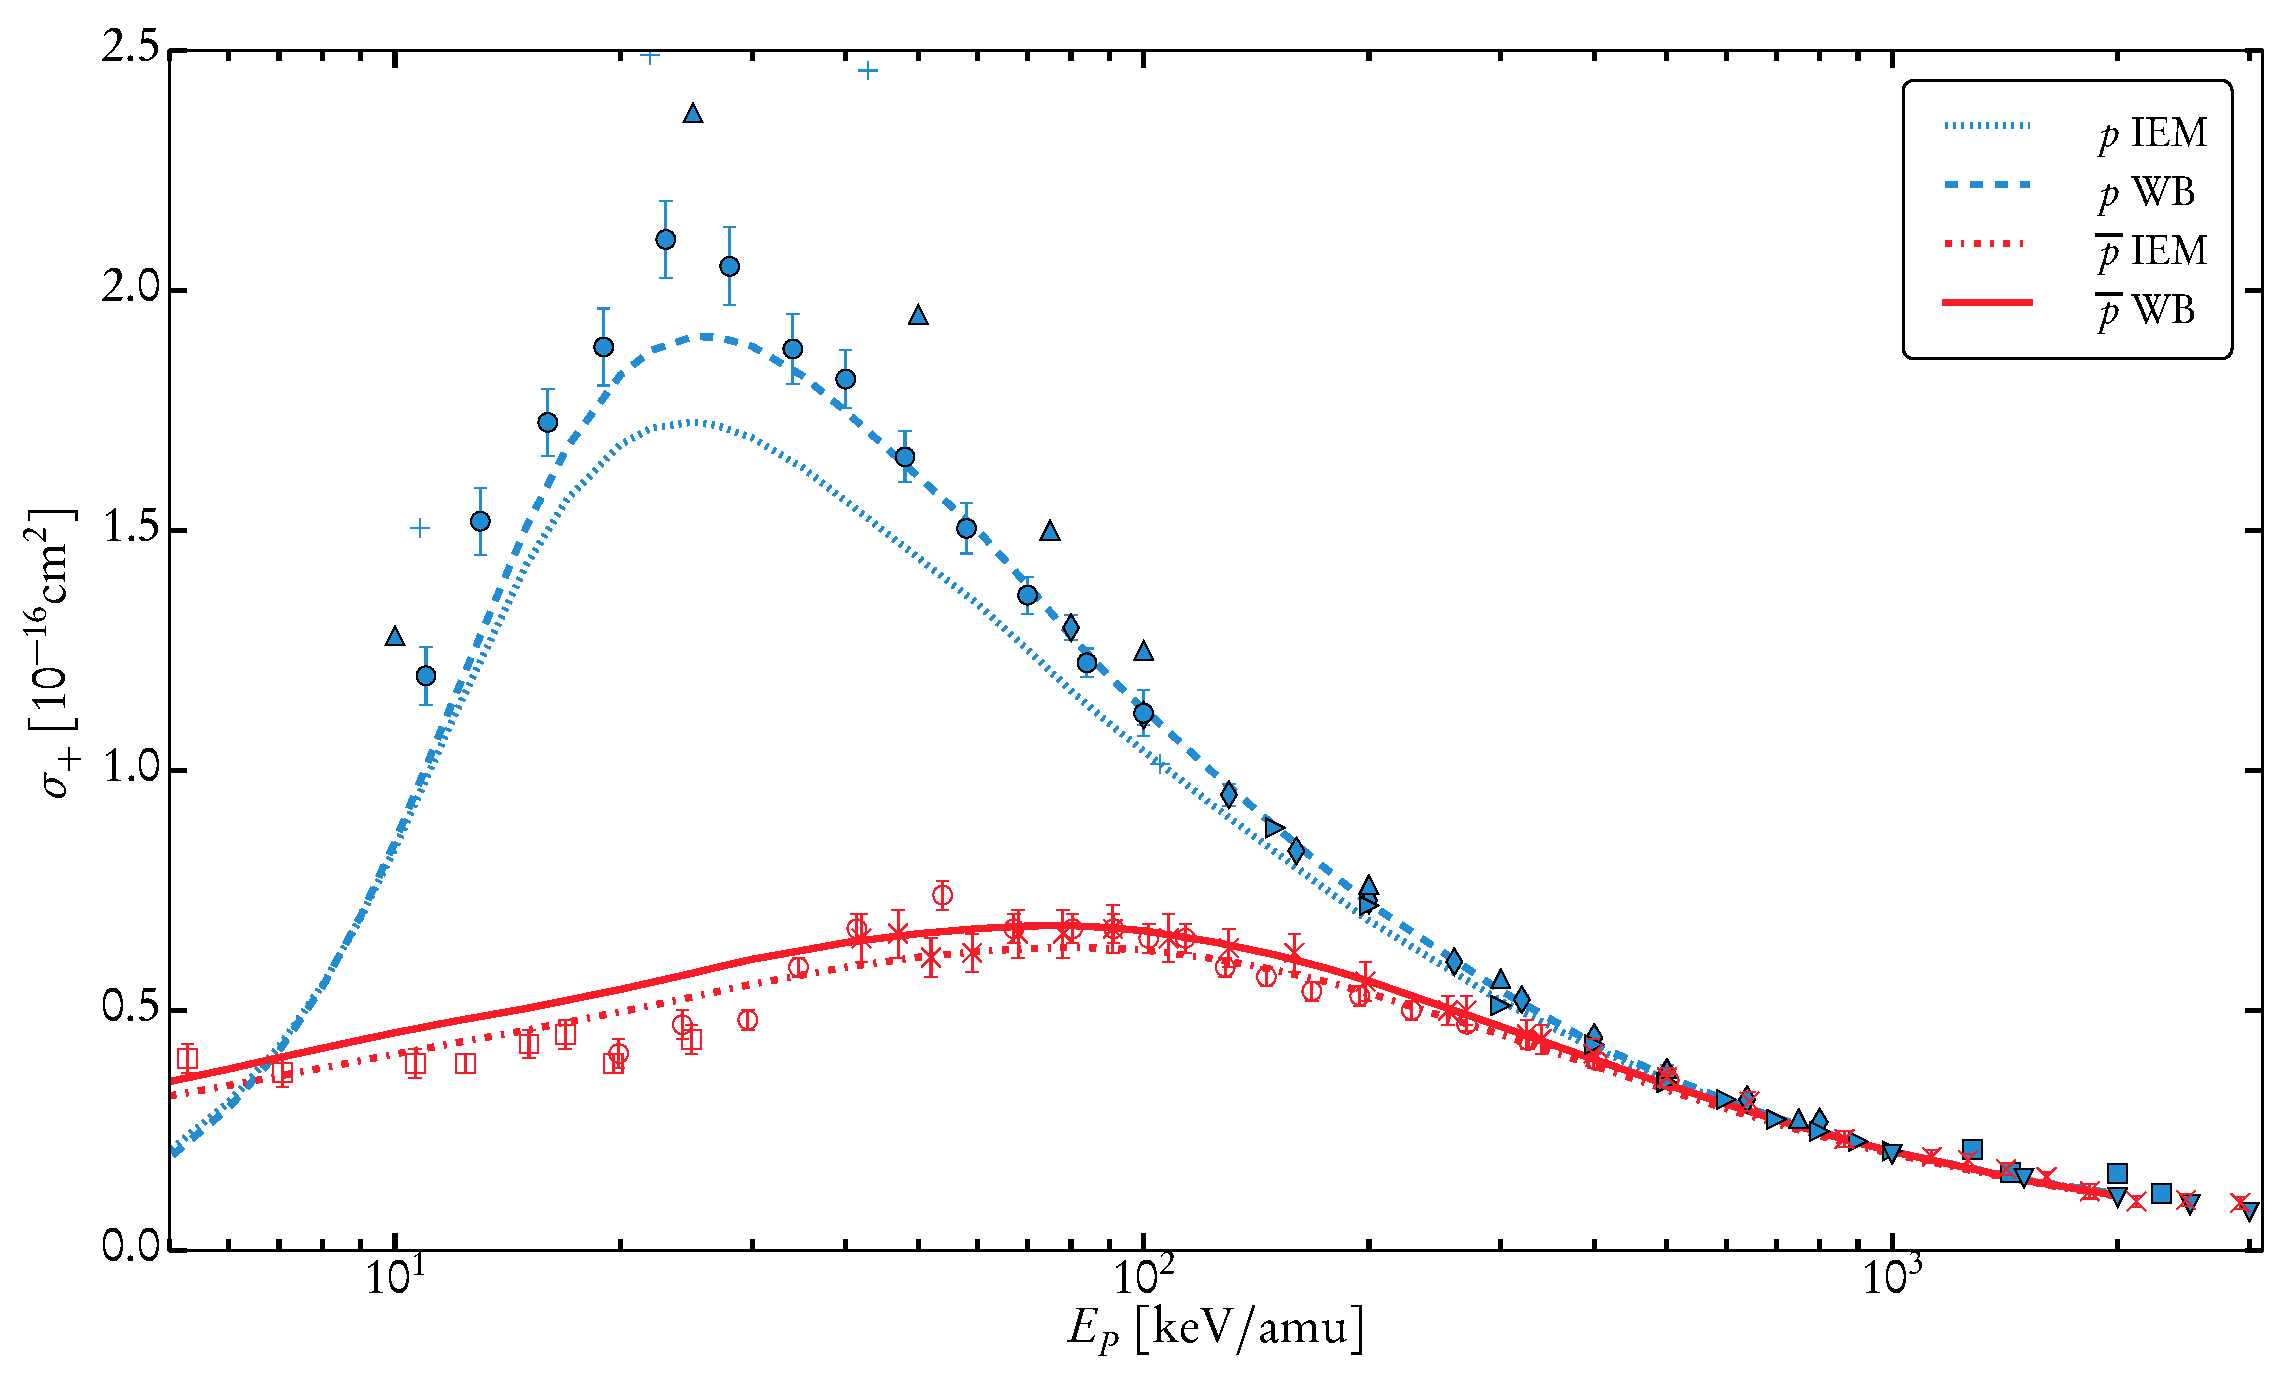
\includegraphics[width = \linewidth]{./images/pbarhe/pbarhe-+.eps}
            \caption[Total cross section for one-electron removal from helium by protons and
                     antiprotons.]
                    {Total cross section for one-electron removal from helium by protons and
                     antiprotons. Protons: dotted IEM, dashed WB (theory);
                     {\color{blue}{$\blacktriangle$}}~\cite{DTR84}, {\color{blue}{$+$}}~\cite{Sol62},
                     {\color{blue}{$\bullet$}}~\cite{SG89}, {\color{blue}{$\blacklozenge$}}~\cite{SG85},
                     {\color{blue}{$\blacktriangleright$}}~\cite{PM70},
                     {\color{blue}{$\blacktriangledown$}}~\cite{Wex64},
                     {\color{blue}{$\blacksquare$}}~\cite{KAH84} (experiment).
                     Antiprotons: dashed-dotted IEM, solid WB (theory);
                     {\color{red}{$\Box$}}~\cite{KKT08}, {\color{red}{$\circ$}}~\cite{HKM94},
                     {\color{red}{$\times$}}~\cite{AHK90} (experiment). \label{fig:he+}}
         \end{figure}
         
         \begin{figure}[htp]
            \centering
            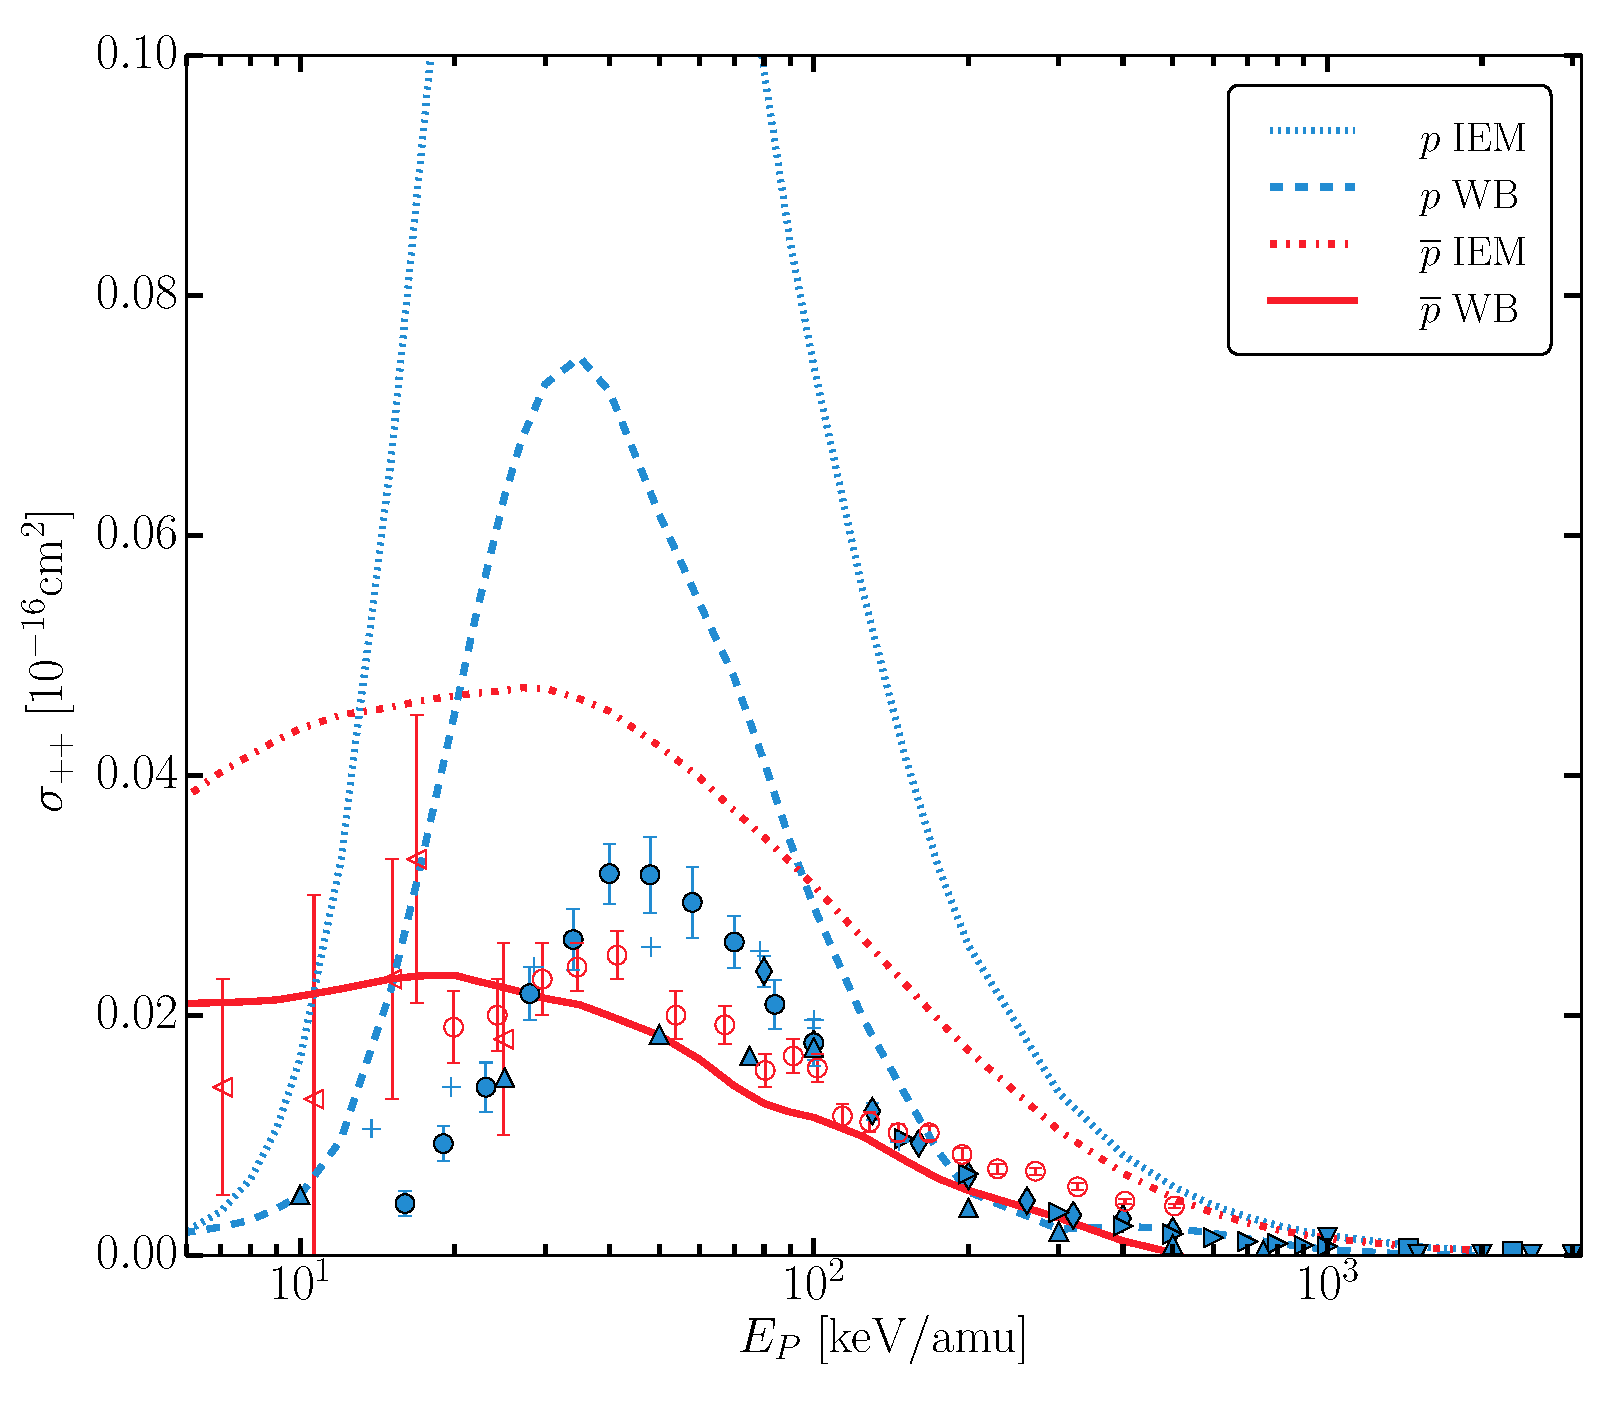
\includegraphics[width = \linewidth]{./images/pbarhe/pbarhe-++.eps}
            \caption[Total cross section for two-electron removal from helium atoms as a function of
                     impact energy]
                    {Total cross section for two-electron removal from helium atoms as a function
                     of impact energy. Protons: dotted IEM, dashed WB (theory);
                     {\color{blue}{$\blacktriangle$}}~\cite{DTR84}, {\color{blue}{$+$}}~\cite{Sol62},
                     {\color{blue}{$\bullet$}}~\cite{SG89}, {\color{blue}{$\blacklozenge$}}~\cite{SG85},
                    {\color{blue}{$\blacktriangleright$}}~\cite{PM70},
                    {\color{blue}{$\blacktriangledown$}}~\cite{Wex64},
                    {\color{blue}{$\blacksquare$}}~\cite{KAH84} (experiment).
                    Antiprotons: dashed-dotted IEM, solid WB (theory);
                    {\color{red}{$\circ$}}~\cite{HKM94}, {\color{red}{$\triangleleft$}}~\cite{KKT09}
                    (experiment). \label{fig:he++}}
         \end{figure}

         \begin{itemize}

            \item p-b and Ic plots for pbar- and p-he systems.

            \item plots of electron loss and single/double ionization.

            \item discussion of results.

         \end{itemize}

      \end{subsection}

      \begin{subsection}{phe \label{sec:phe-res}}

         \begin{figure}[htp]
            \centering
            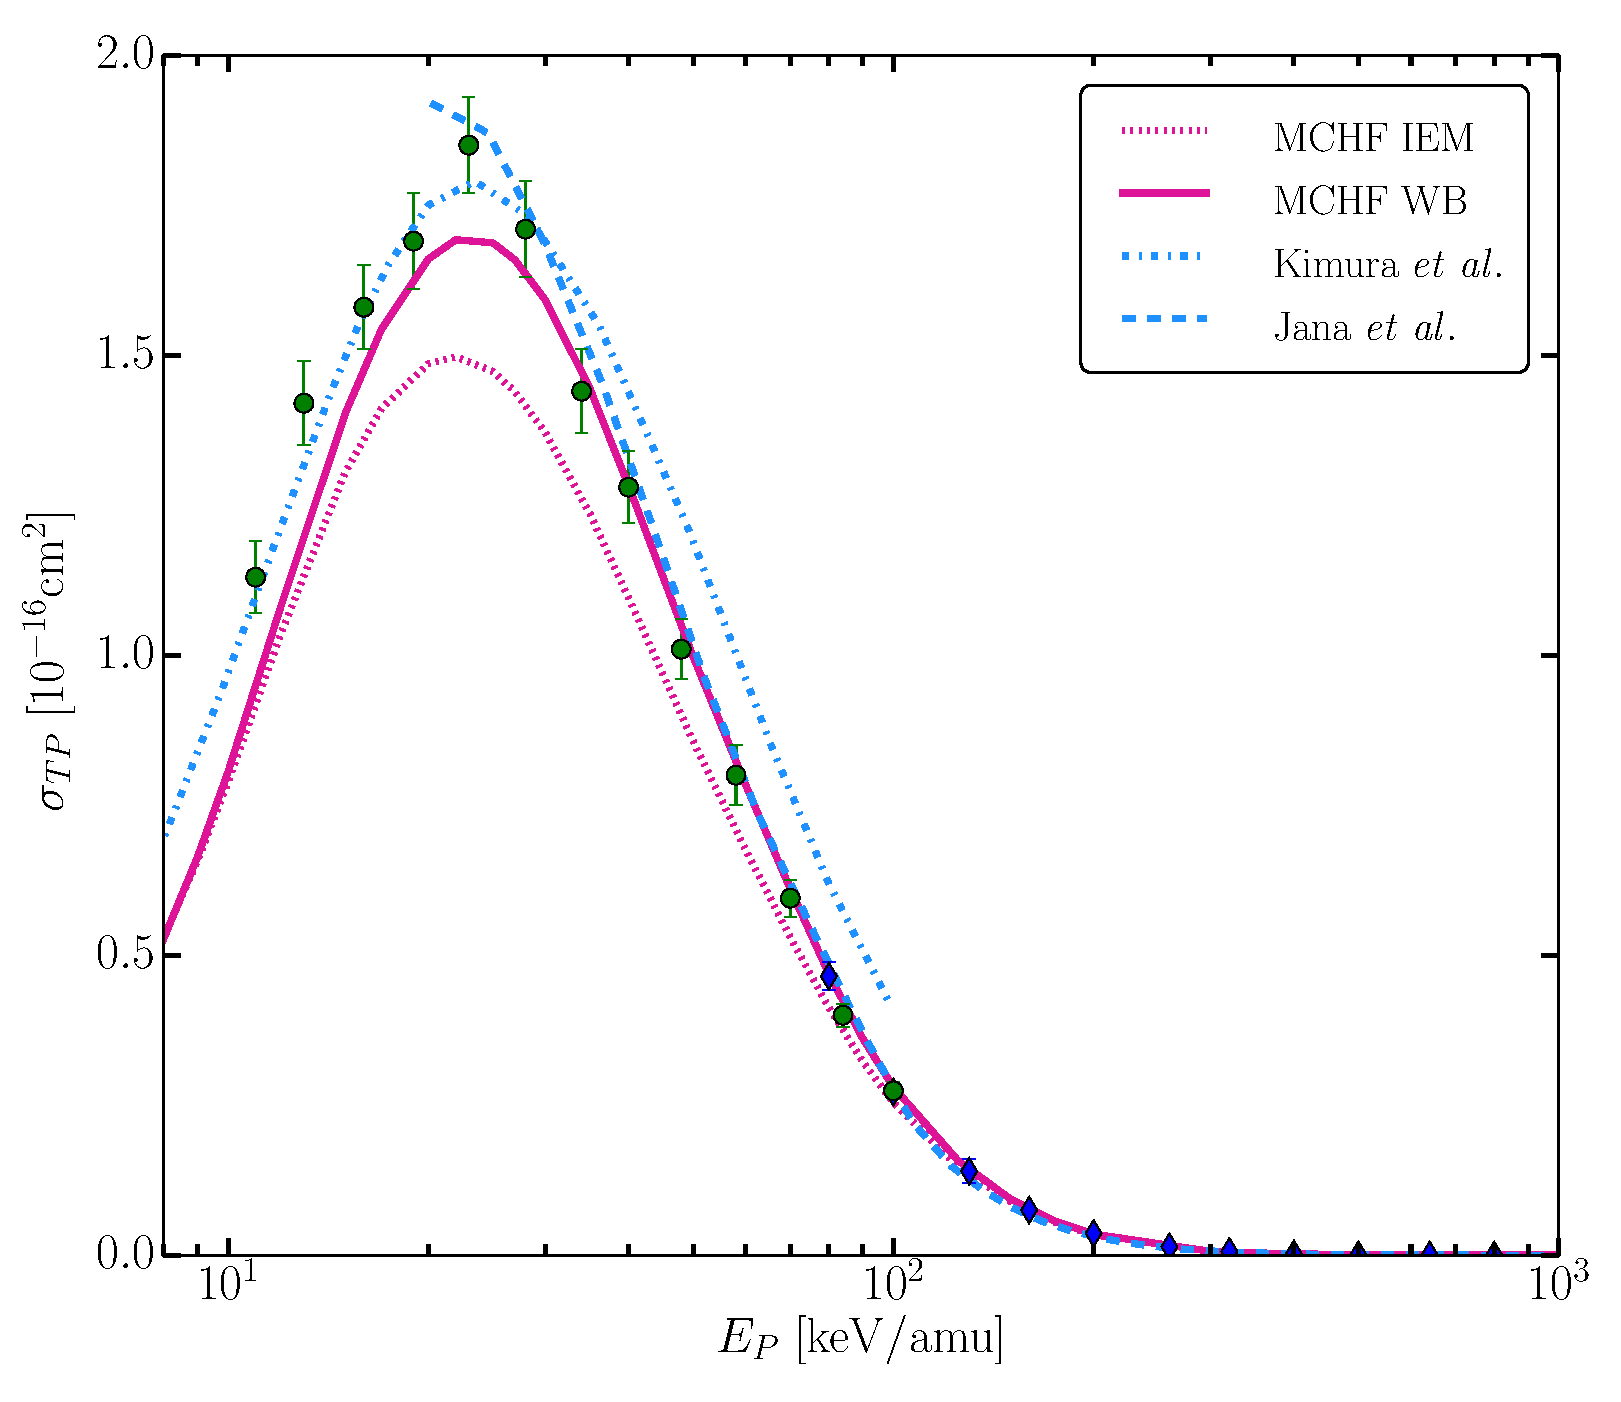
\includegraphics[width = \linewidth]{./images/phe/phe-TP.eps}
            \caption[Total cross section for single capture in proton-helium collisions.]
                    {Total cross section for single capture in proton-helium collisions.
                     Theoretical results: AO-MO model of Kimura \textit{et al}.\ \cite{KL-86} and DW-4B
                     (post form) of Jana \textit{et al}.~\cite{JMP-15}. Experimental Data:
                     {\color{OliveGreen}{$\bullet$}}~\cite{SG89} and
                     {\color{blue}{$\blacklozenge$}}~\cite{SG85}. \label{fig:phe-tp}}
         \end{figure}
         
         \begin{figure}[htp]
            \centering
            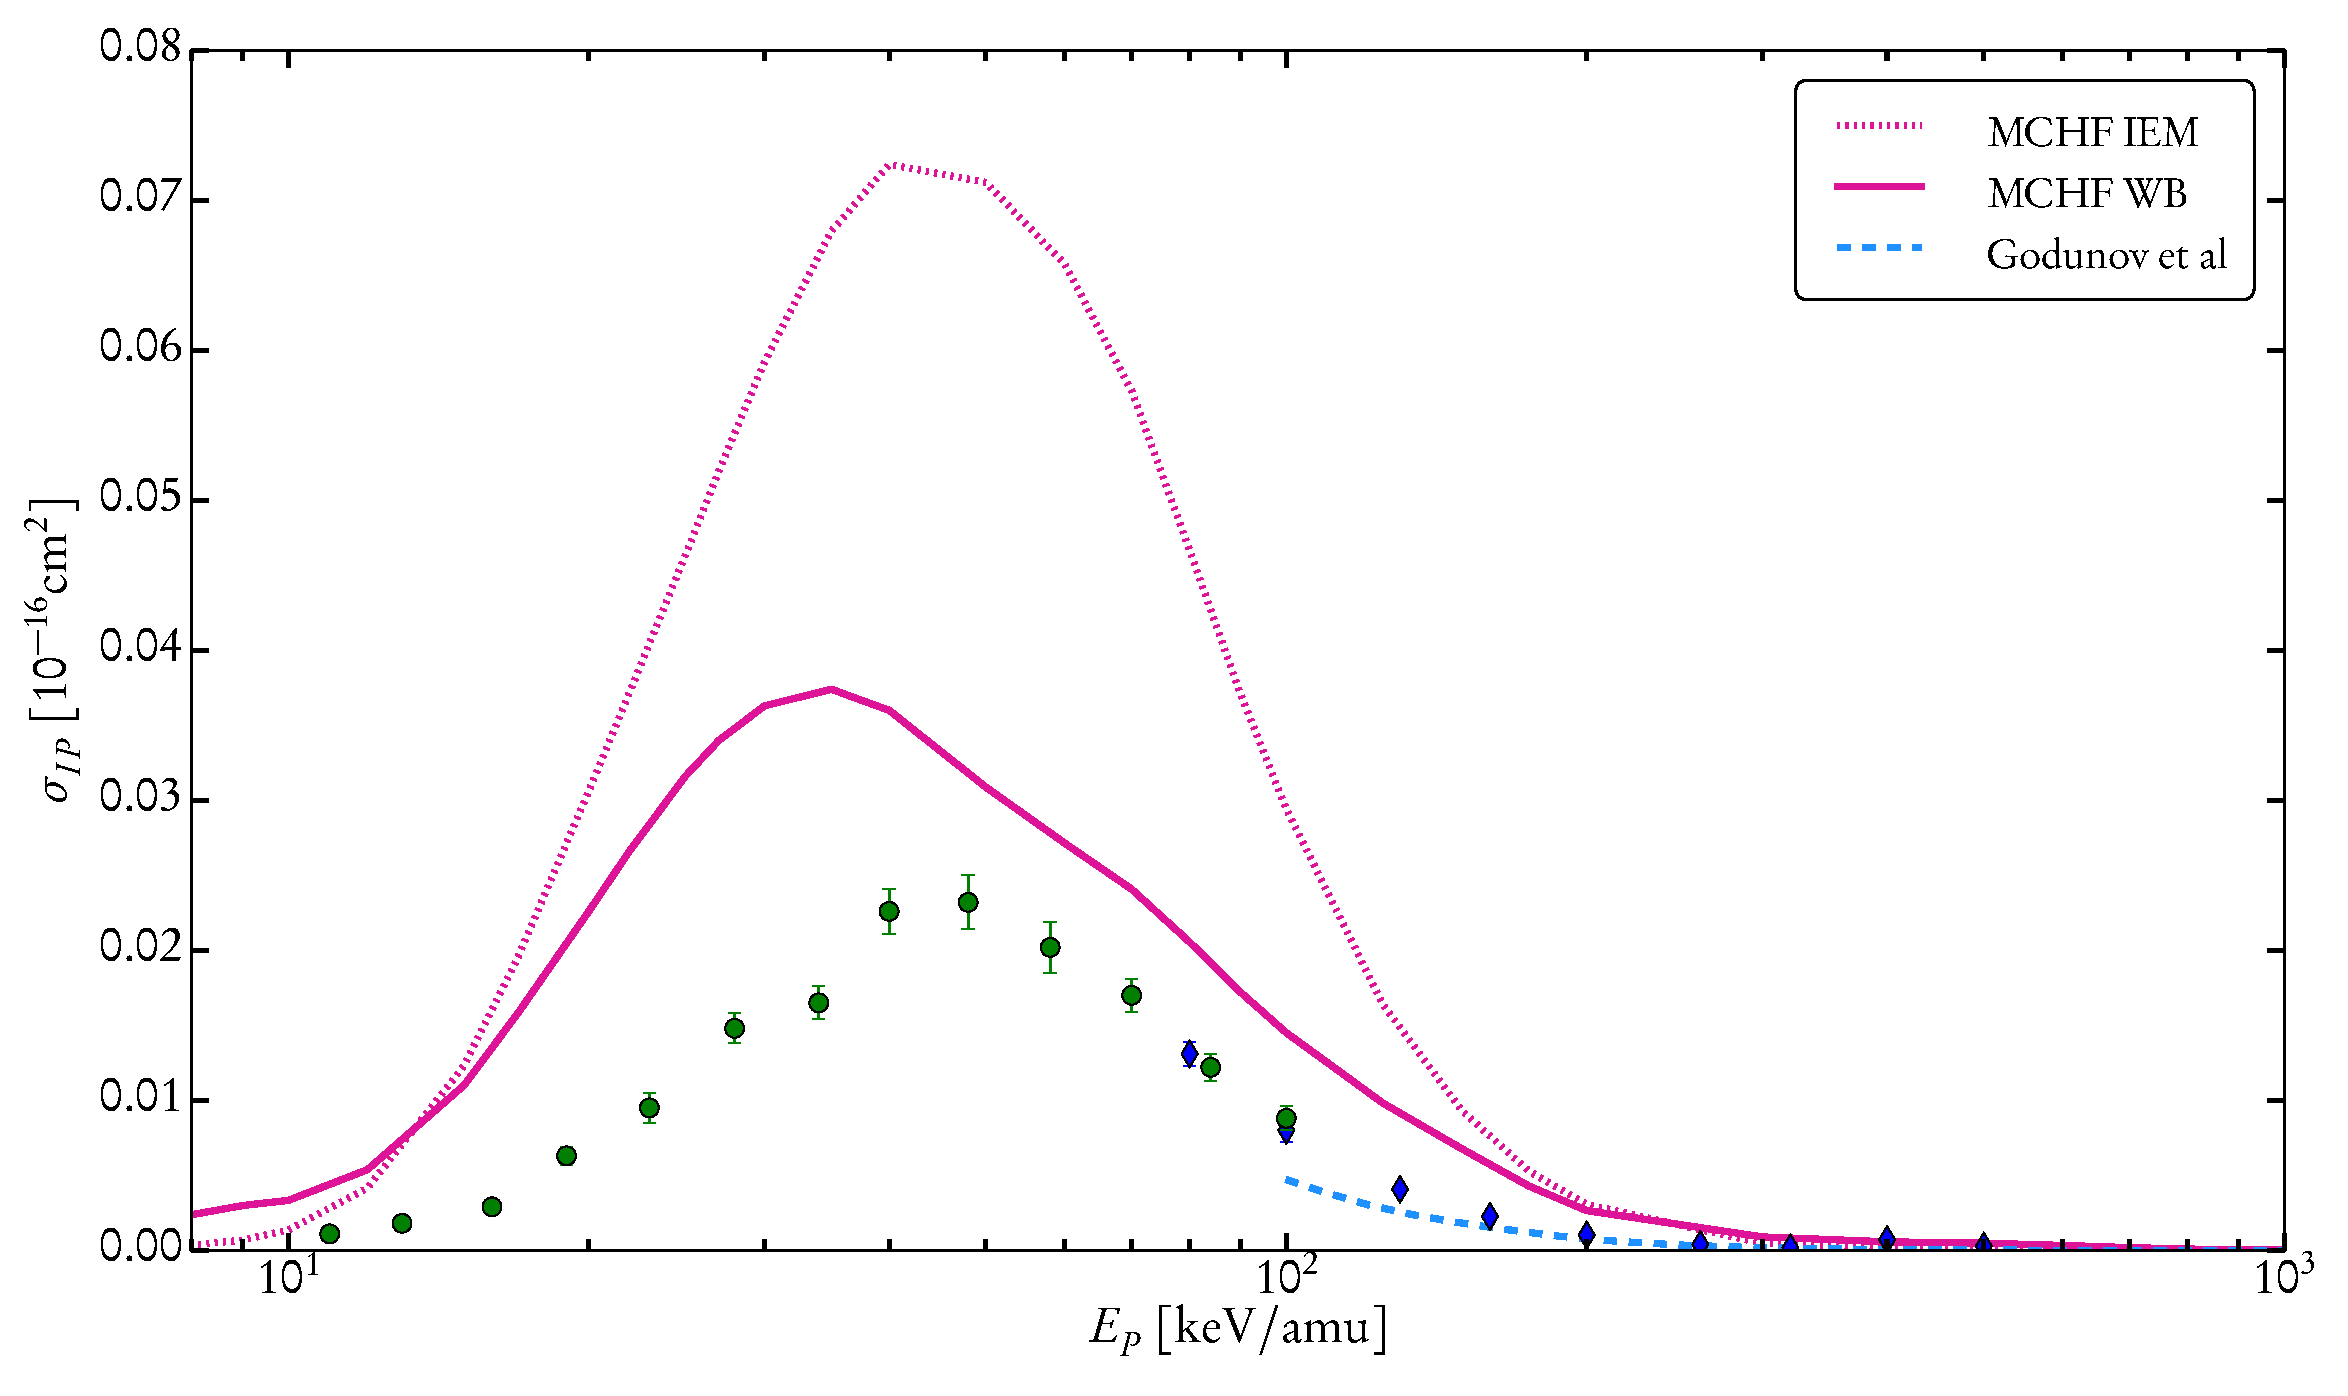
\includegraphics[width = \linewidth]{./images/phe/phe-IP.eps}
            \caption[Total cross section for transfer ionization in proton-helium collisions.]
                    {Total cross section for transfer ionization in proton-helium collisions.
                     Theoretical results: Second order Born approximation of Godunov
                     \textit{et al}.~\cite{Godunov-06}. Experimental data:
                     {\color{OliveGreen}{$\bullet$}}~\cite{SG89} and
                     {\color{blue}{$\blacklozenge$}}~\cite{SG85}. \label{fig:phe-ip}}
         \end{figure}
         
         \begin{figure}[htp]
            \centering
            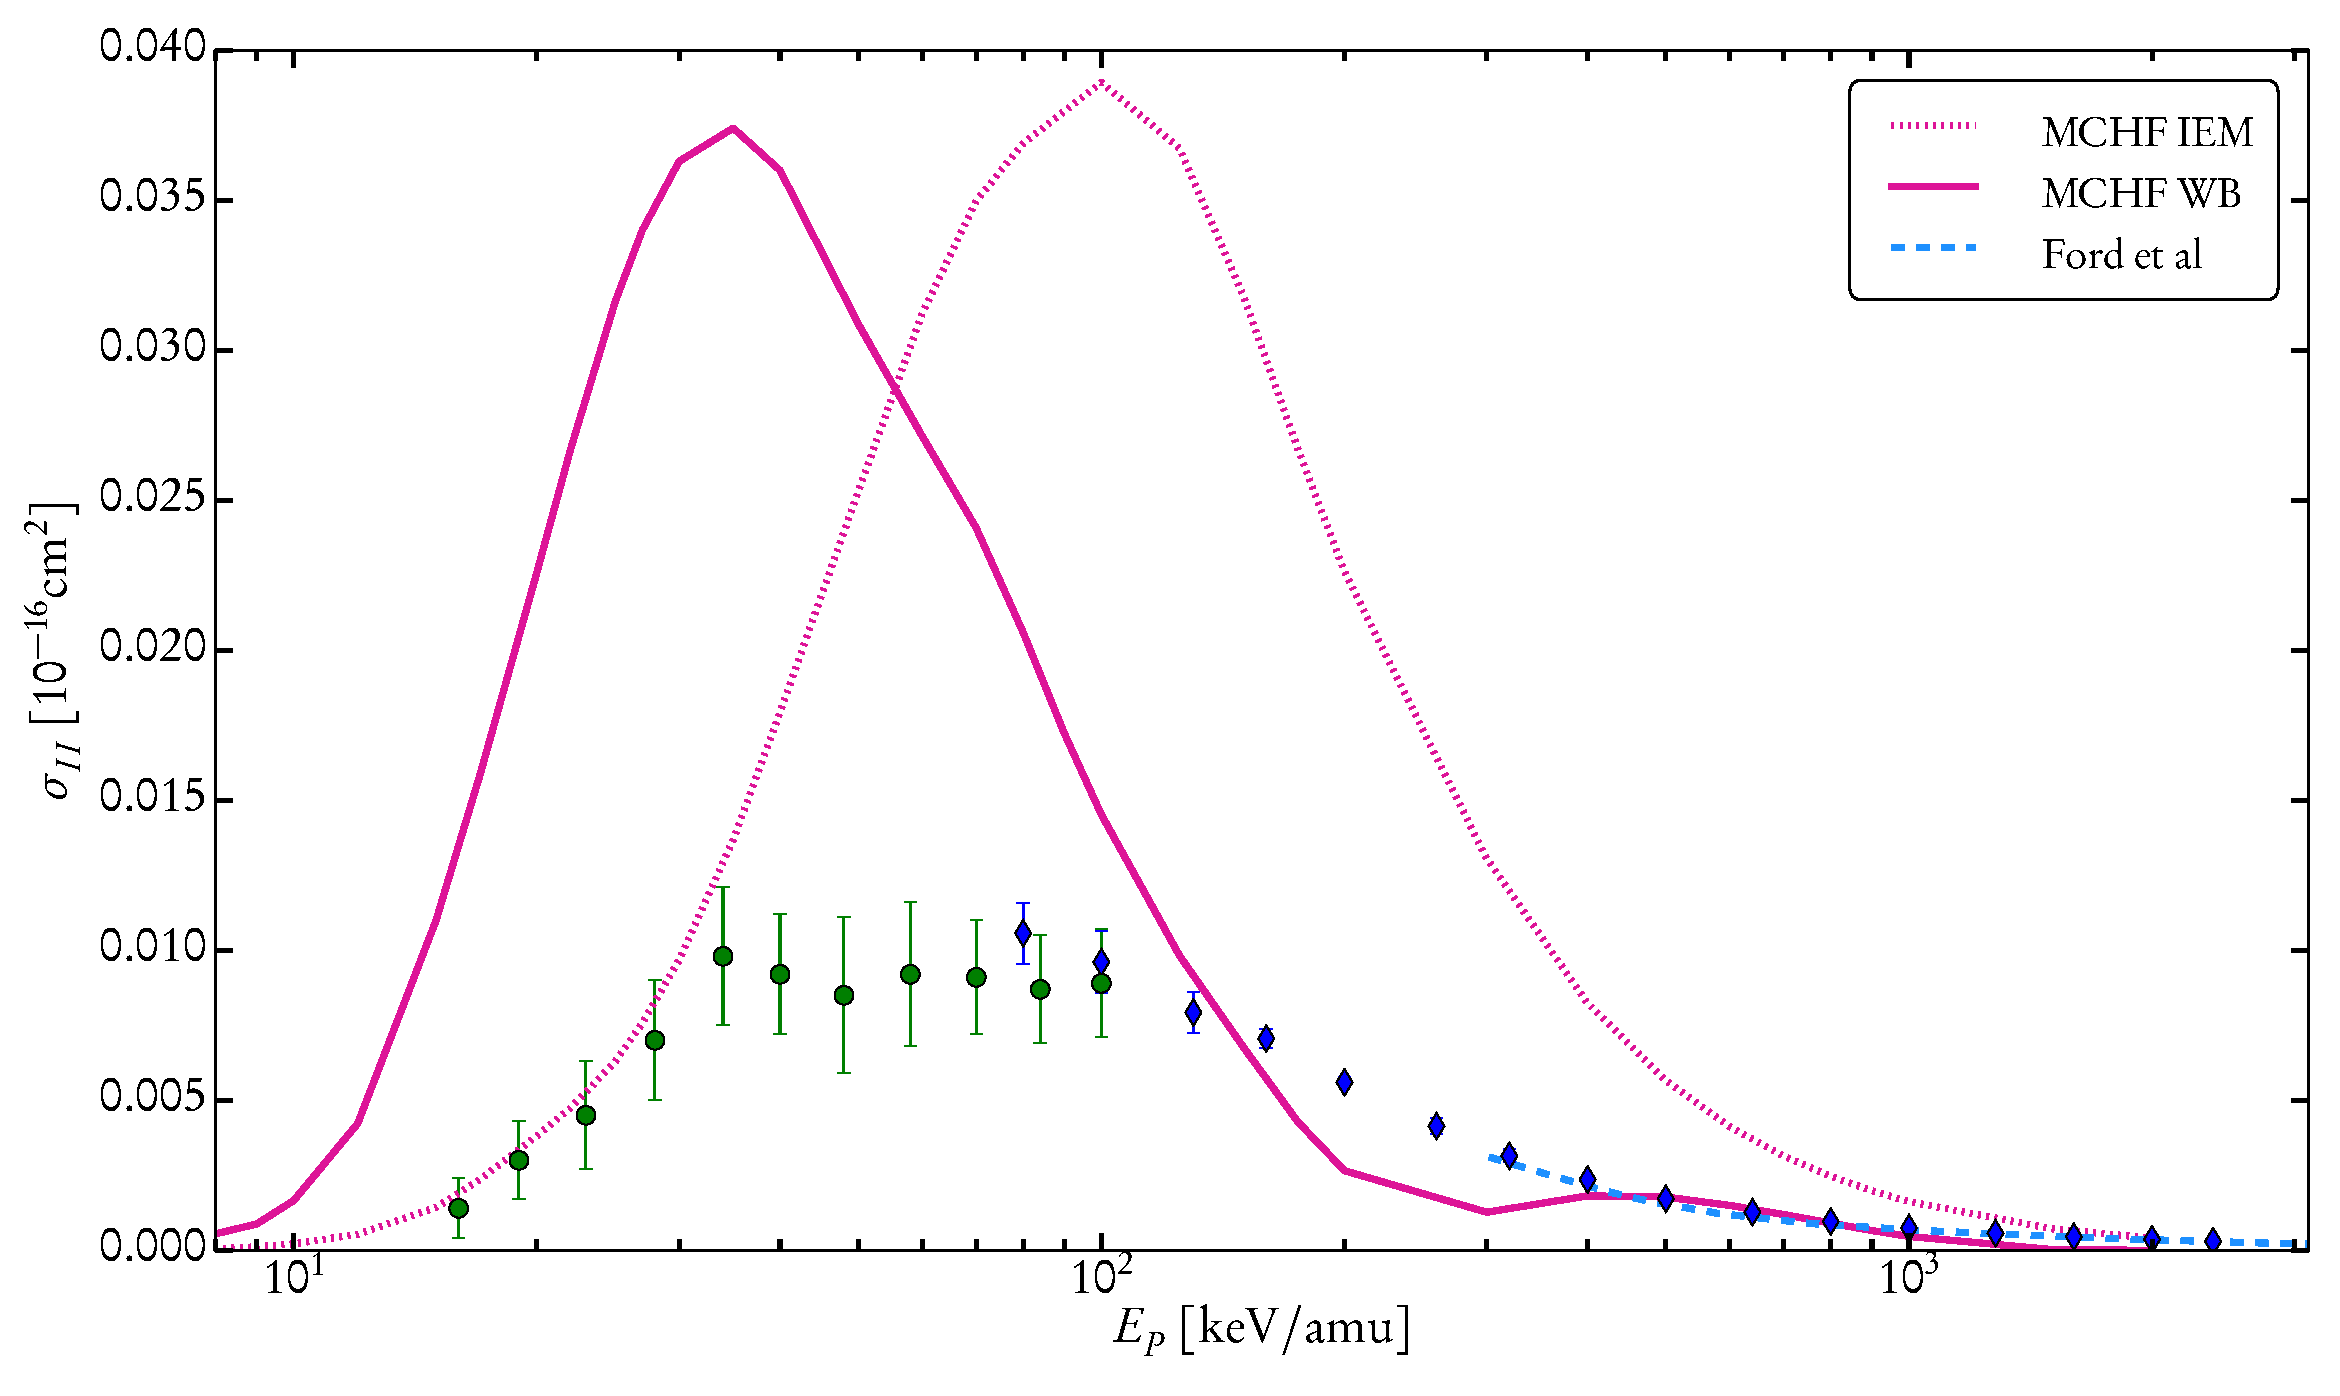
\includegraphics[width = \linewidth]{./images/phe/phe-II.eps}
            \caption[Total cross section for double ionization of helium by proton impact.]
                    {Total cross section for double ionization of helium by proton impact.
                     Theoretical results: FIM of Ford \textit{et al}.~\cite{FR-94}
                     Experimental data: {\color{OliveGreen}{$\bullet$}}~\cite{SG89} and
                     {\color{blue}{$\blacklozenge$}}~\cite{SG85}. \label{fig:phe-ii}}
         \end{figure}
         
         \begin{figure}[htp]
            \centering
            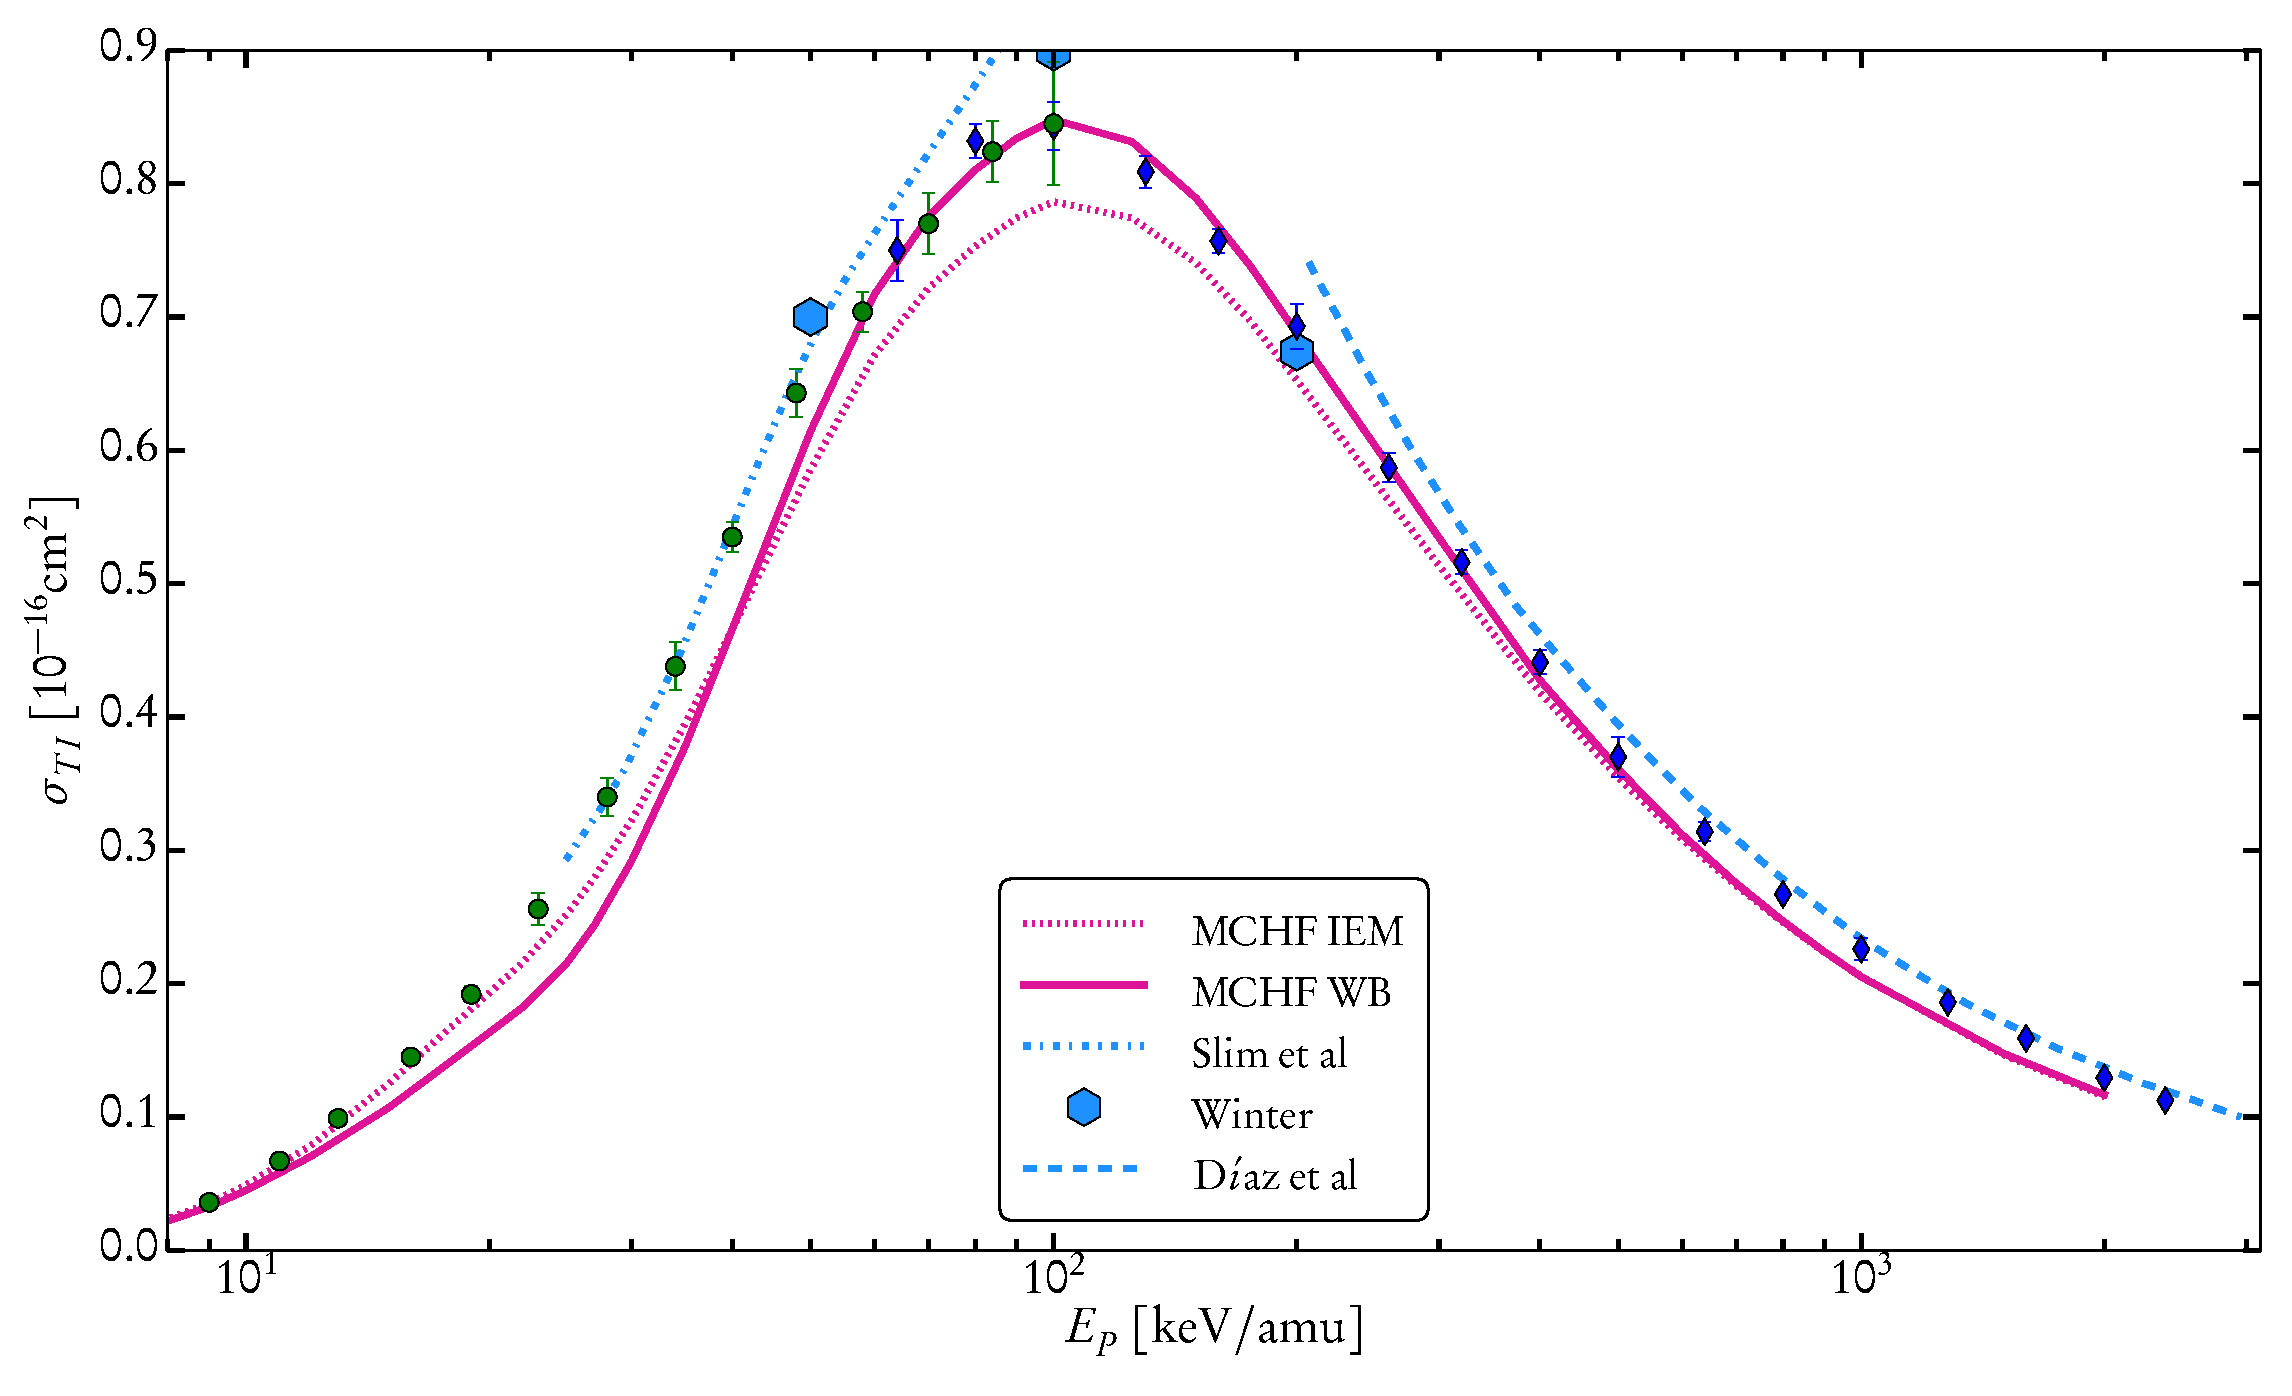
\includegraphics[width = \linewidth]{./images/phe/phe-TI.eps}
            \caption[Total cross section for single ionization of helium by proton impact.]
                    {Total cross section for single ionization of helium by proton impact.
                     Theoretical results: Slim \textit{et al}.~\cite{SHBF-91}, Winter~\cite{Winter-91}
                     D\'{i}az \textit{et al}.~\cite{DMS-00}
                     Experimental data: {\color{OliveGreen}{$\bullet$}}~\cite{SG89} and
                     {\color{blue}{$\blacklozenge$}}~\cite{SG85}. \label{fig:phe-ti}}
         \end{figure}

      \end{subsection}

      \begin{subsection}{he2phe \label{sec:he2phe-res}}

         \begin{figure}[htp]
            \centering
            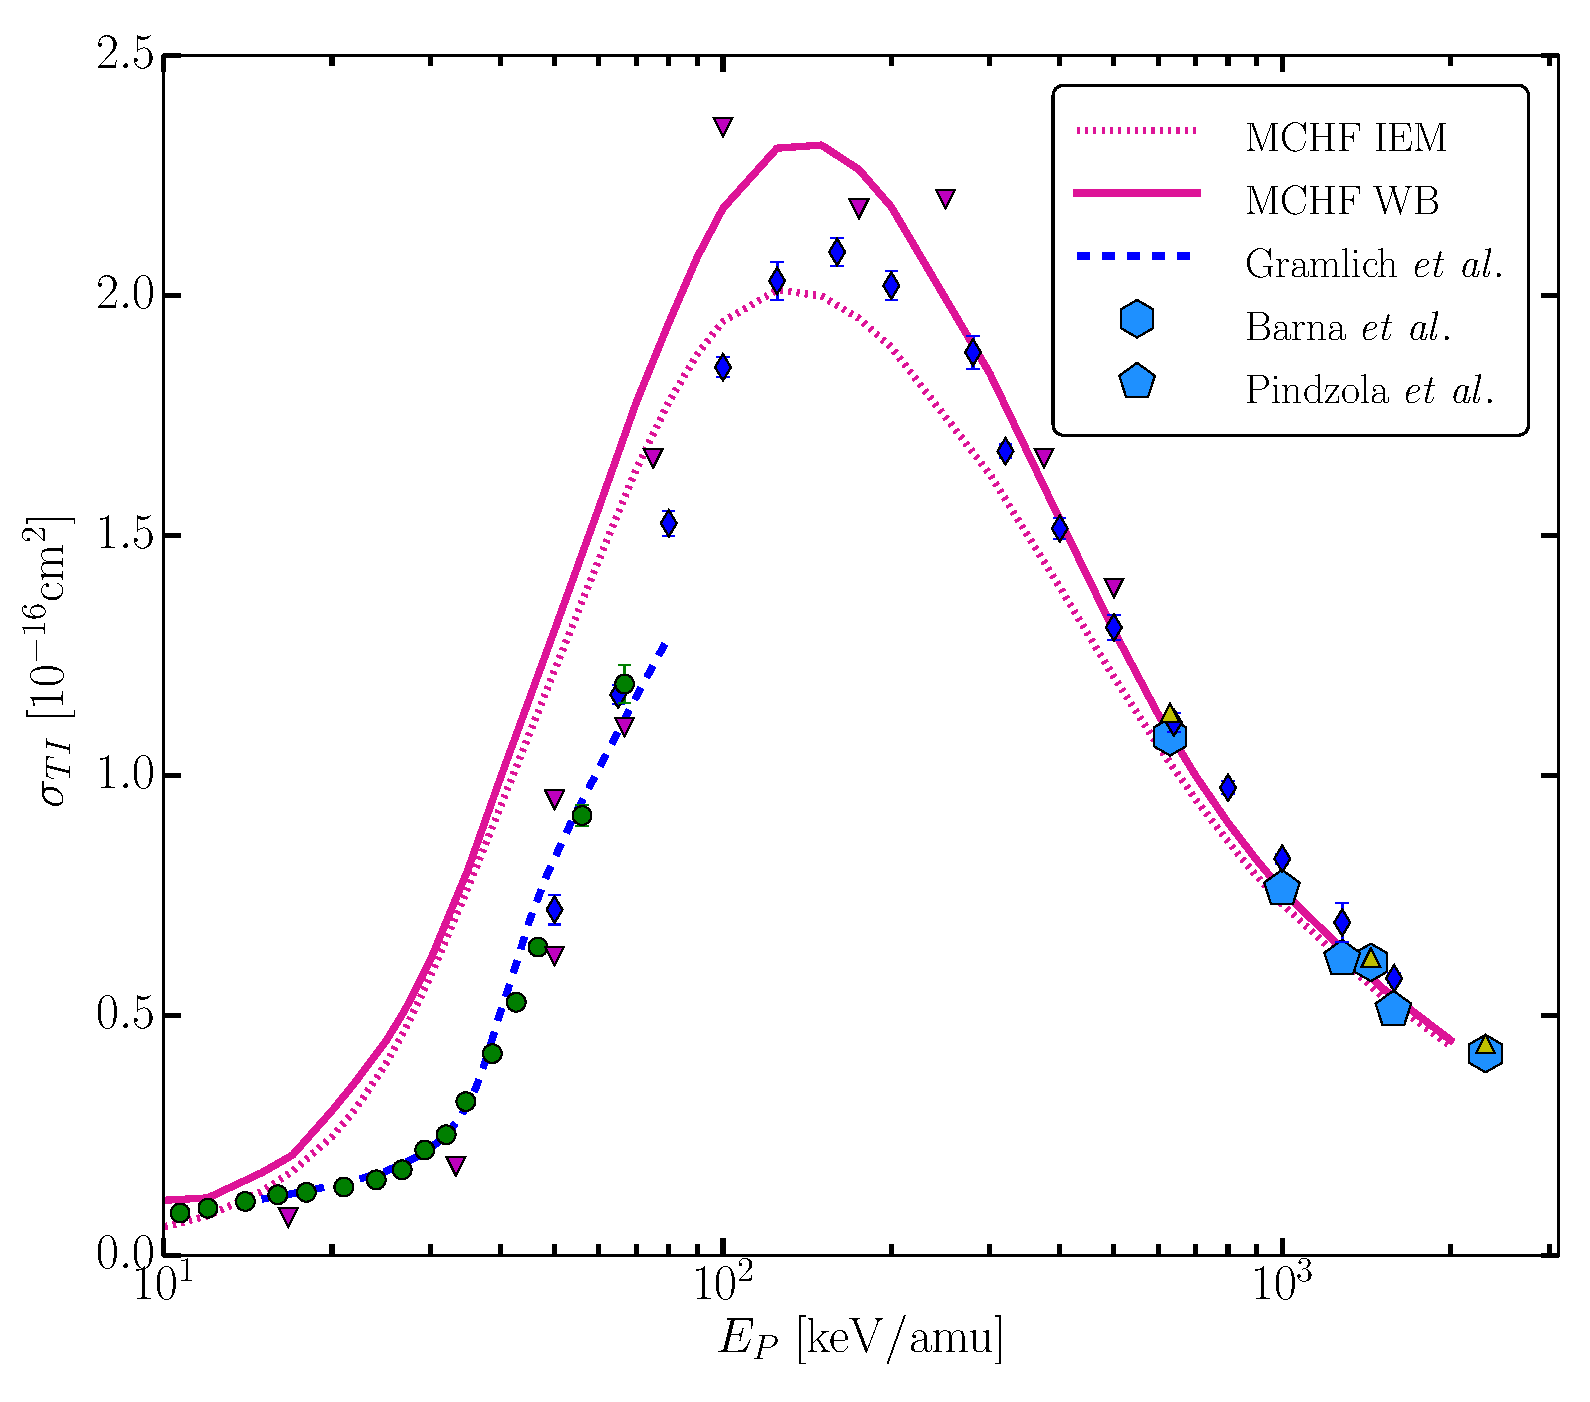
\includegraphics[width = \linewidth]{./images/he2phe/he2phe-TI.eps}
            \caption[Total cross section for single ionization of helium by He\textsuperscript{2+}
                     impact.]{Total cross section for single ionization of helium by
                     He\textsuperscript{2+} impact. Theoretical results: Gramlich
                     \textit{et al}.~\cite{GGS-89}, Barna
                     \textit{et al}.~\cite{BTB-05}, Pindzola \textit{et al}.~\cite{PRC-07}.
                     Experimental data: {\color{blue}{$\blacklozenge$}}~\cite{SG85},
                     {\color{OliveGreen}{$\bullet$}}~\cite{SG89},
                     {\color{RedViolet}{$\blacktriangledown$}}~\cite{Dubois87},
                     {\color{GreenYellow}$\blacktriangle$}~\cite{KAH84}. \label{fig:he2phe-ti}}
         \end{figure}
         
         \begin{figure}[htp]
            \centering
            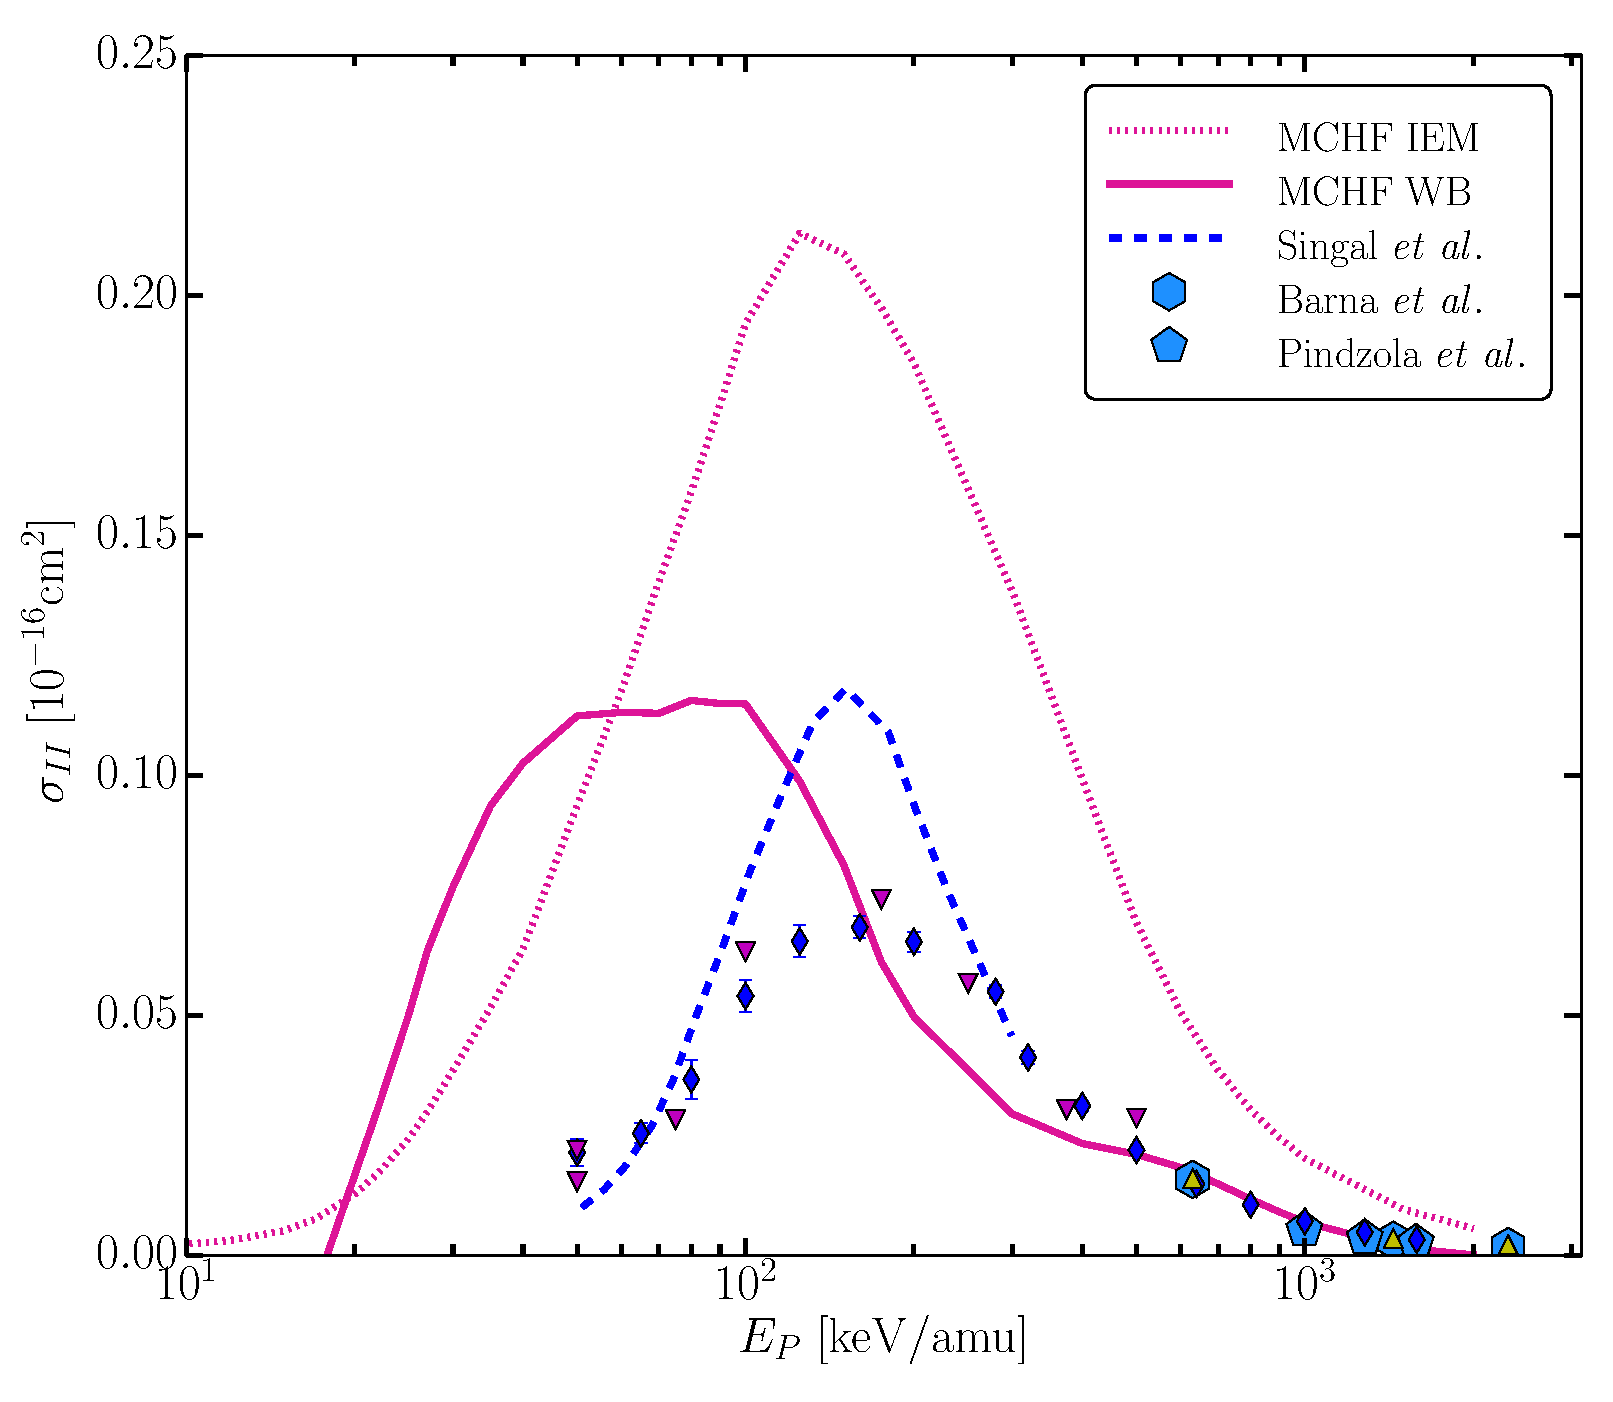
\includegraphics[width = \linewidth]{./images/he2phe/he2phe-II.eps}
            \caption[Total cross section for double ionization of helium by He\textsuperscript{2+}
                     impact.]{Total cross section for double ionization of helium by
                     He\textsuperscript{2+} impact. Theoretical results: Singal
                     \textit{et al}.~\cite{SL-91}, Barna
                     \textit{et al}.~\cite{BTB-05}, Pindzola \textit{et al}.~\cite{PRC-07}
                     Experimental data: {\color{blue}{$\blacklozenge$}}~\cite{SG85},
                     {\color{RedViolet}{$\blacktriangledown$}}~\cite{Dubois87},
                     {\color{GreenYellow}$\blacktriangle$}~\cite{KAH84}. \label{fig:he2phe-ii}}
         \end{figure}
         
         \begin{figure}[htp]
            \centering
            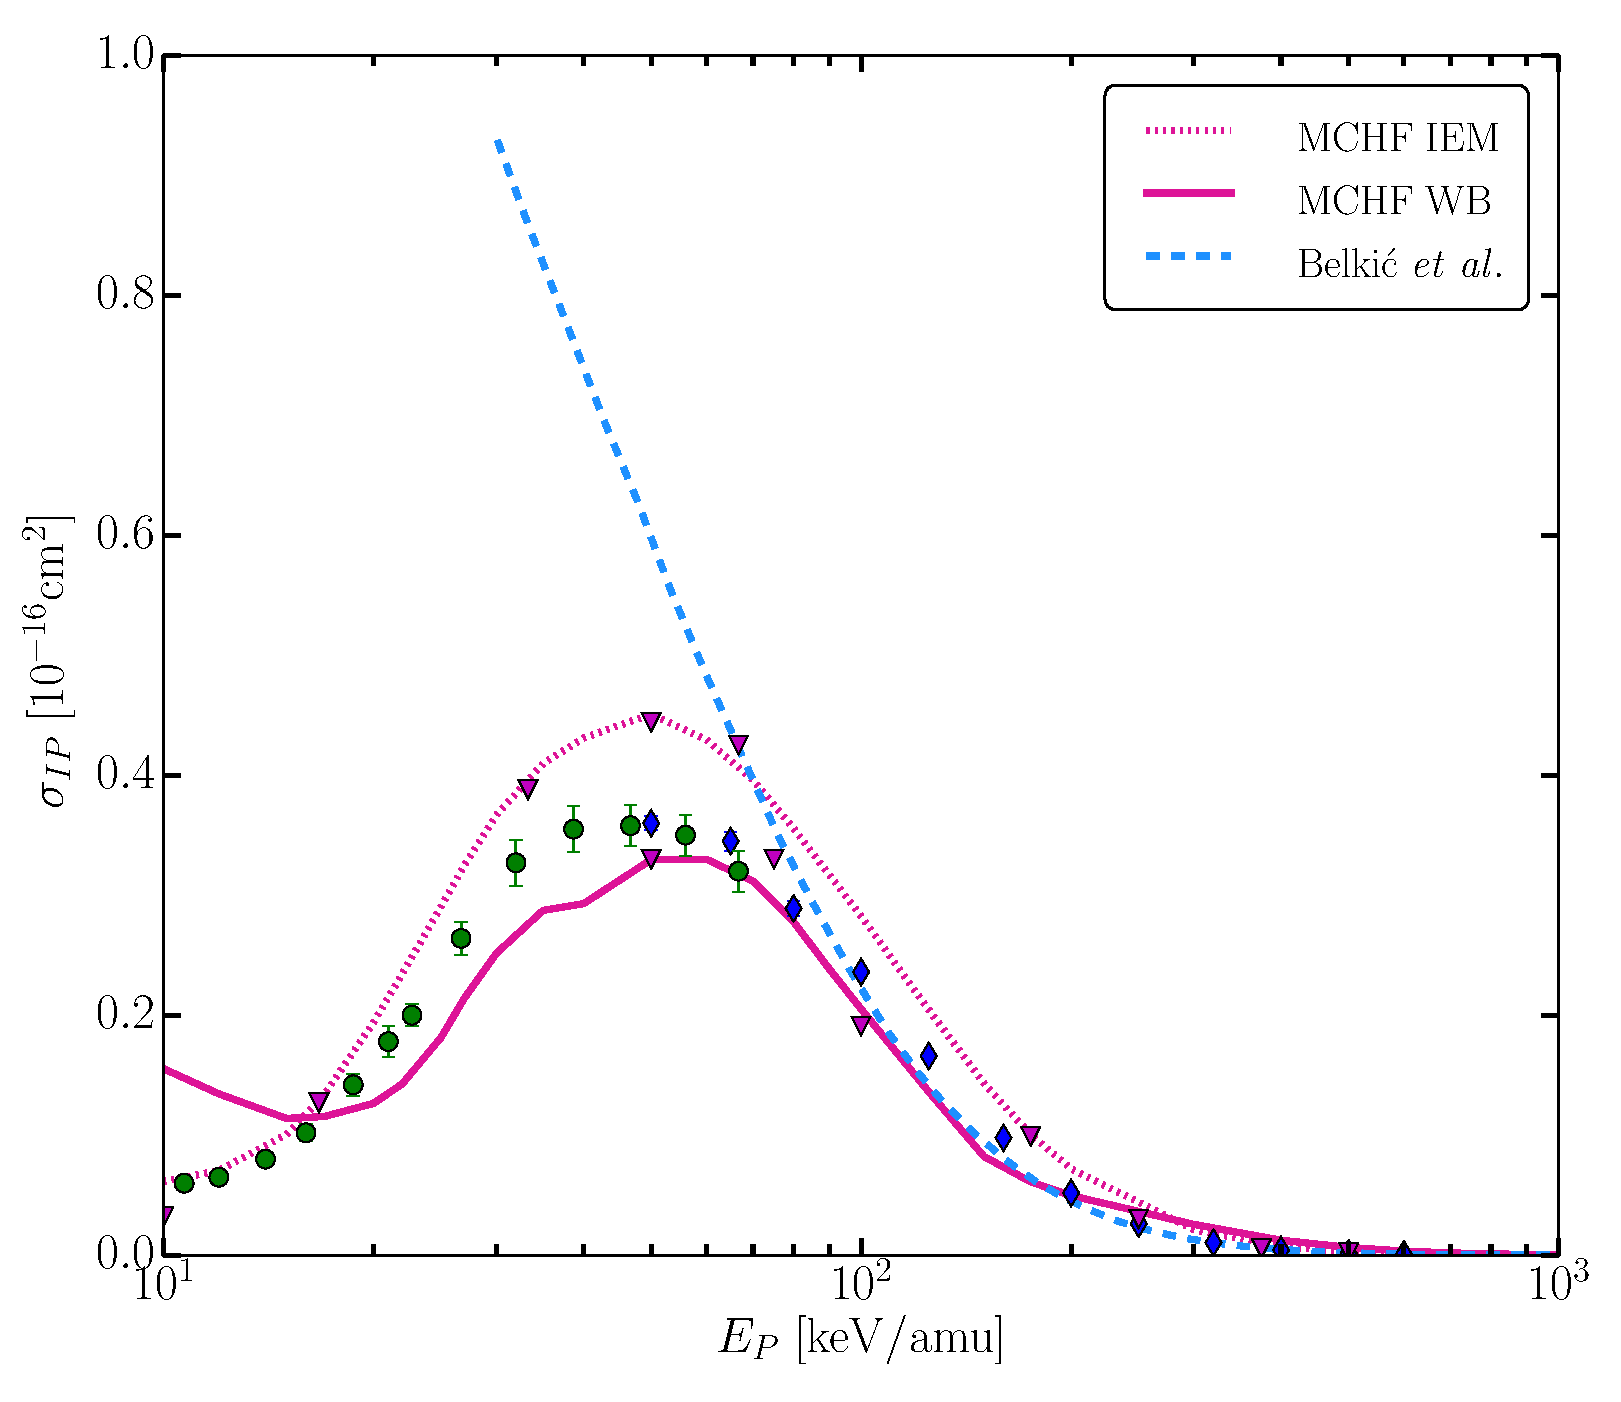
\includegraphics[width = \linewidth]{./images/he2phe/he2phe-IP.eps}
            \caption[Total cross section for transfer ionization in He\textsuperscript{2+}-He
                     Collisions.]{Total cross section for transfer ionization in
                     He\textsuperscript{2+}-He Collisions. Theoretical results: Belki\'{c}
                     \textit{et al}.~\cite{BMM-97}.
                     Experimental data: {\color{blue}{$\blacklozenge$}}~\cite{SG85},
                     {\color{OliveGreen}{$\bullet$}}~\cite{SG89},
                     {\color{RedViolet}{$\blacktriangledown$}}~\cite{Dubois87}. \label{fig:he2phe-ip}}
         \end{figure}
         
         \begin{figure}[htp]
            \centering
            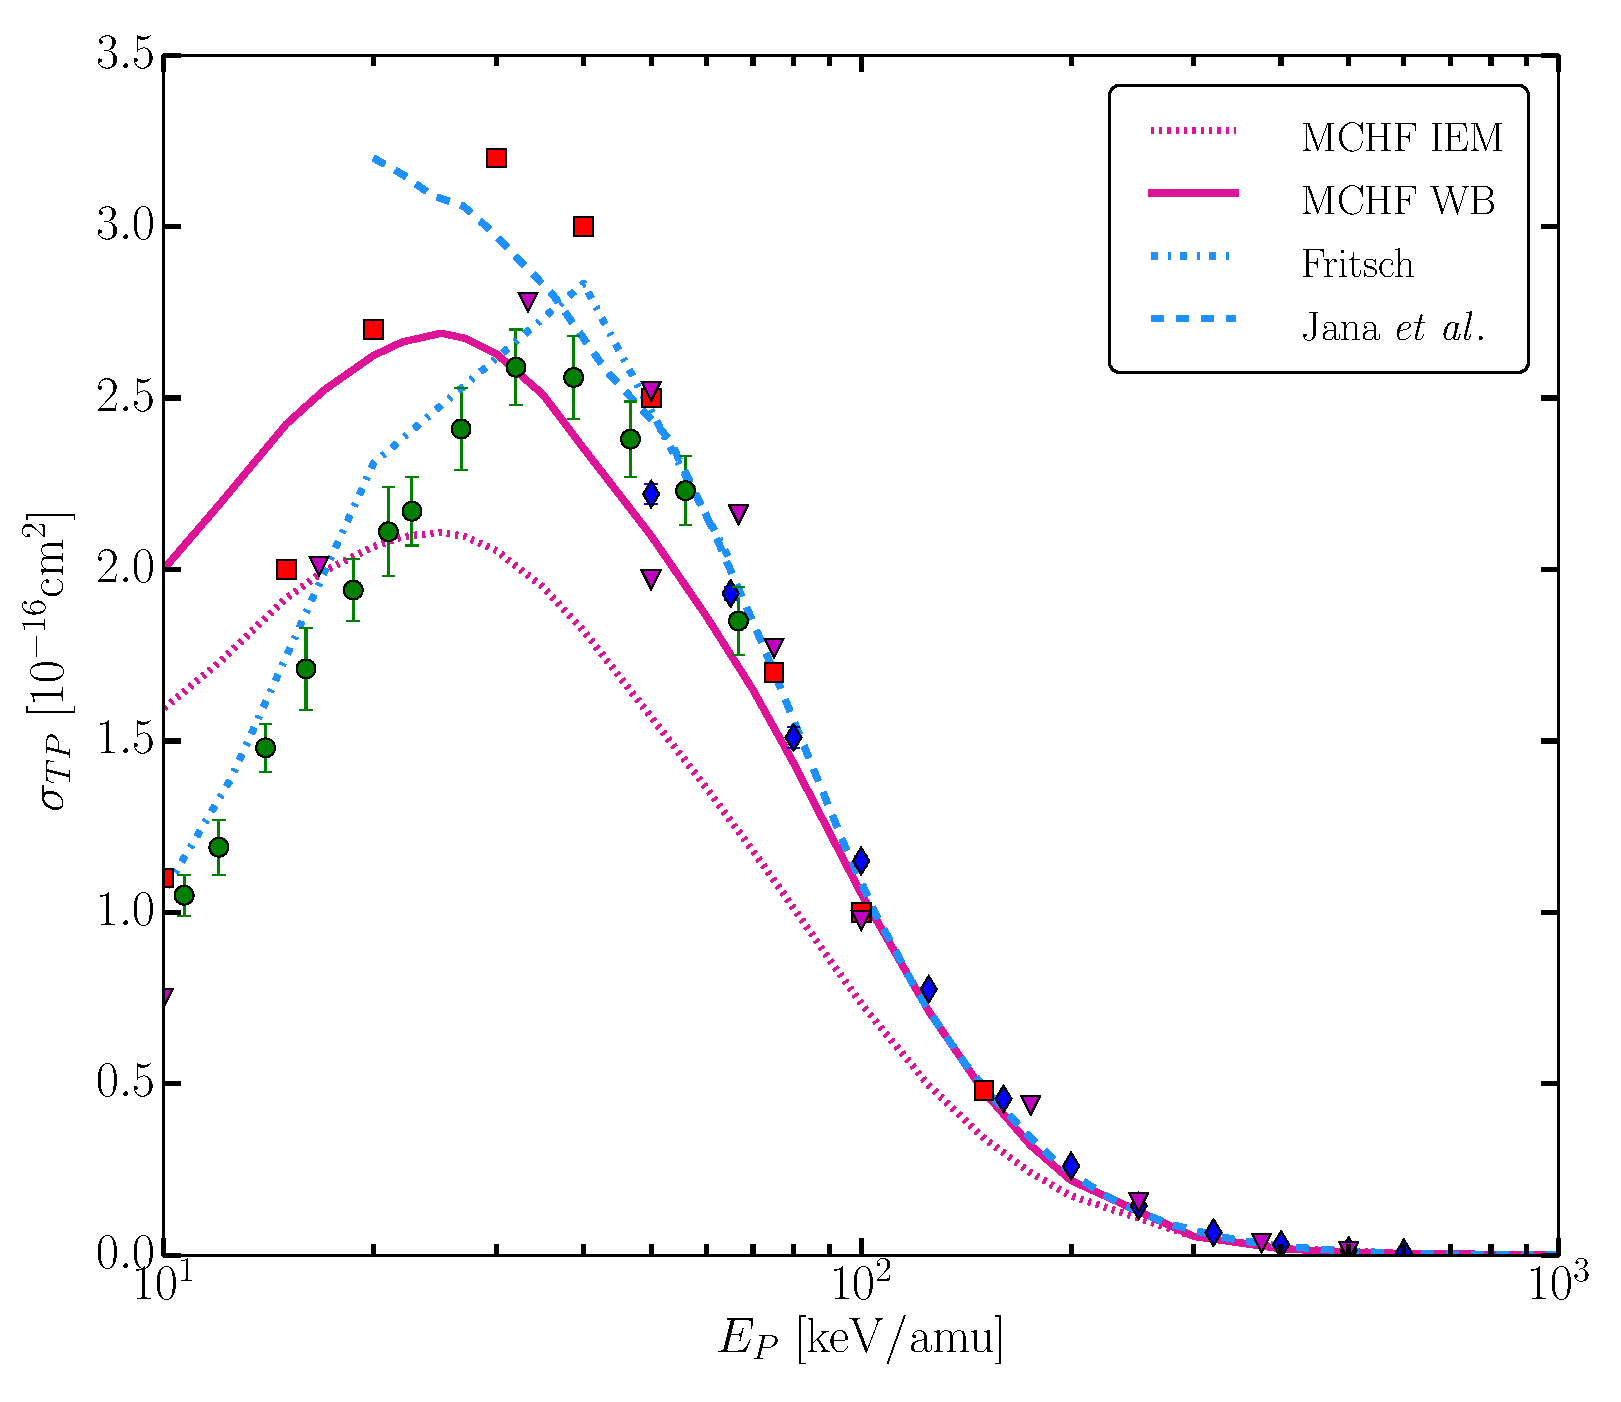
\includegraphics[width = \linewidth]{./images/he2phe/he2phe-TP.eps}
            \caption[Total cross section for single capture in He\textsuperscript{2+}-He
                     collisions.]{Total cross section for single capture in He\textsuperscript{2+}-He
                     collisions. Theoretical results: Fritsch~\cite{Fritsch-94} and DW-4B of Jana
                     \textit{et al}.~\cite{JMP-15}.
                     Experimental data: {\color{blue}{$\blacklozenge$}}~\cite{SG85},
                     {\color{OliveGreen}{$\bullet$}}~\cite{SG89},
                     {\color{RedViolet}{$\blacktriangledown$}}~\cite{Dubois87},
                     {\color{red}$\blacksquare$}~\cite{Rudd85}. \label{fig:he2phe-tp}}
         \end{figure}
         
         \begin{figure}[htp]
            \centering
            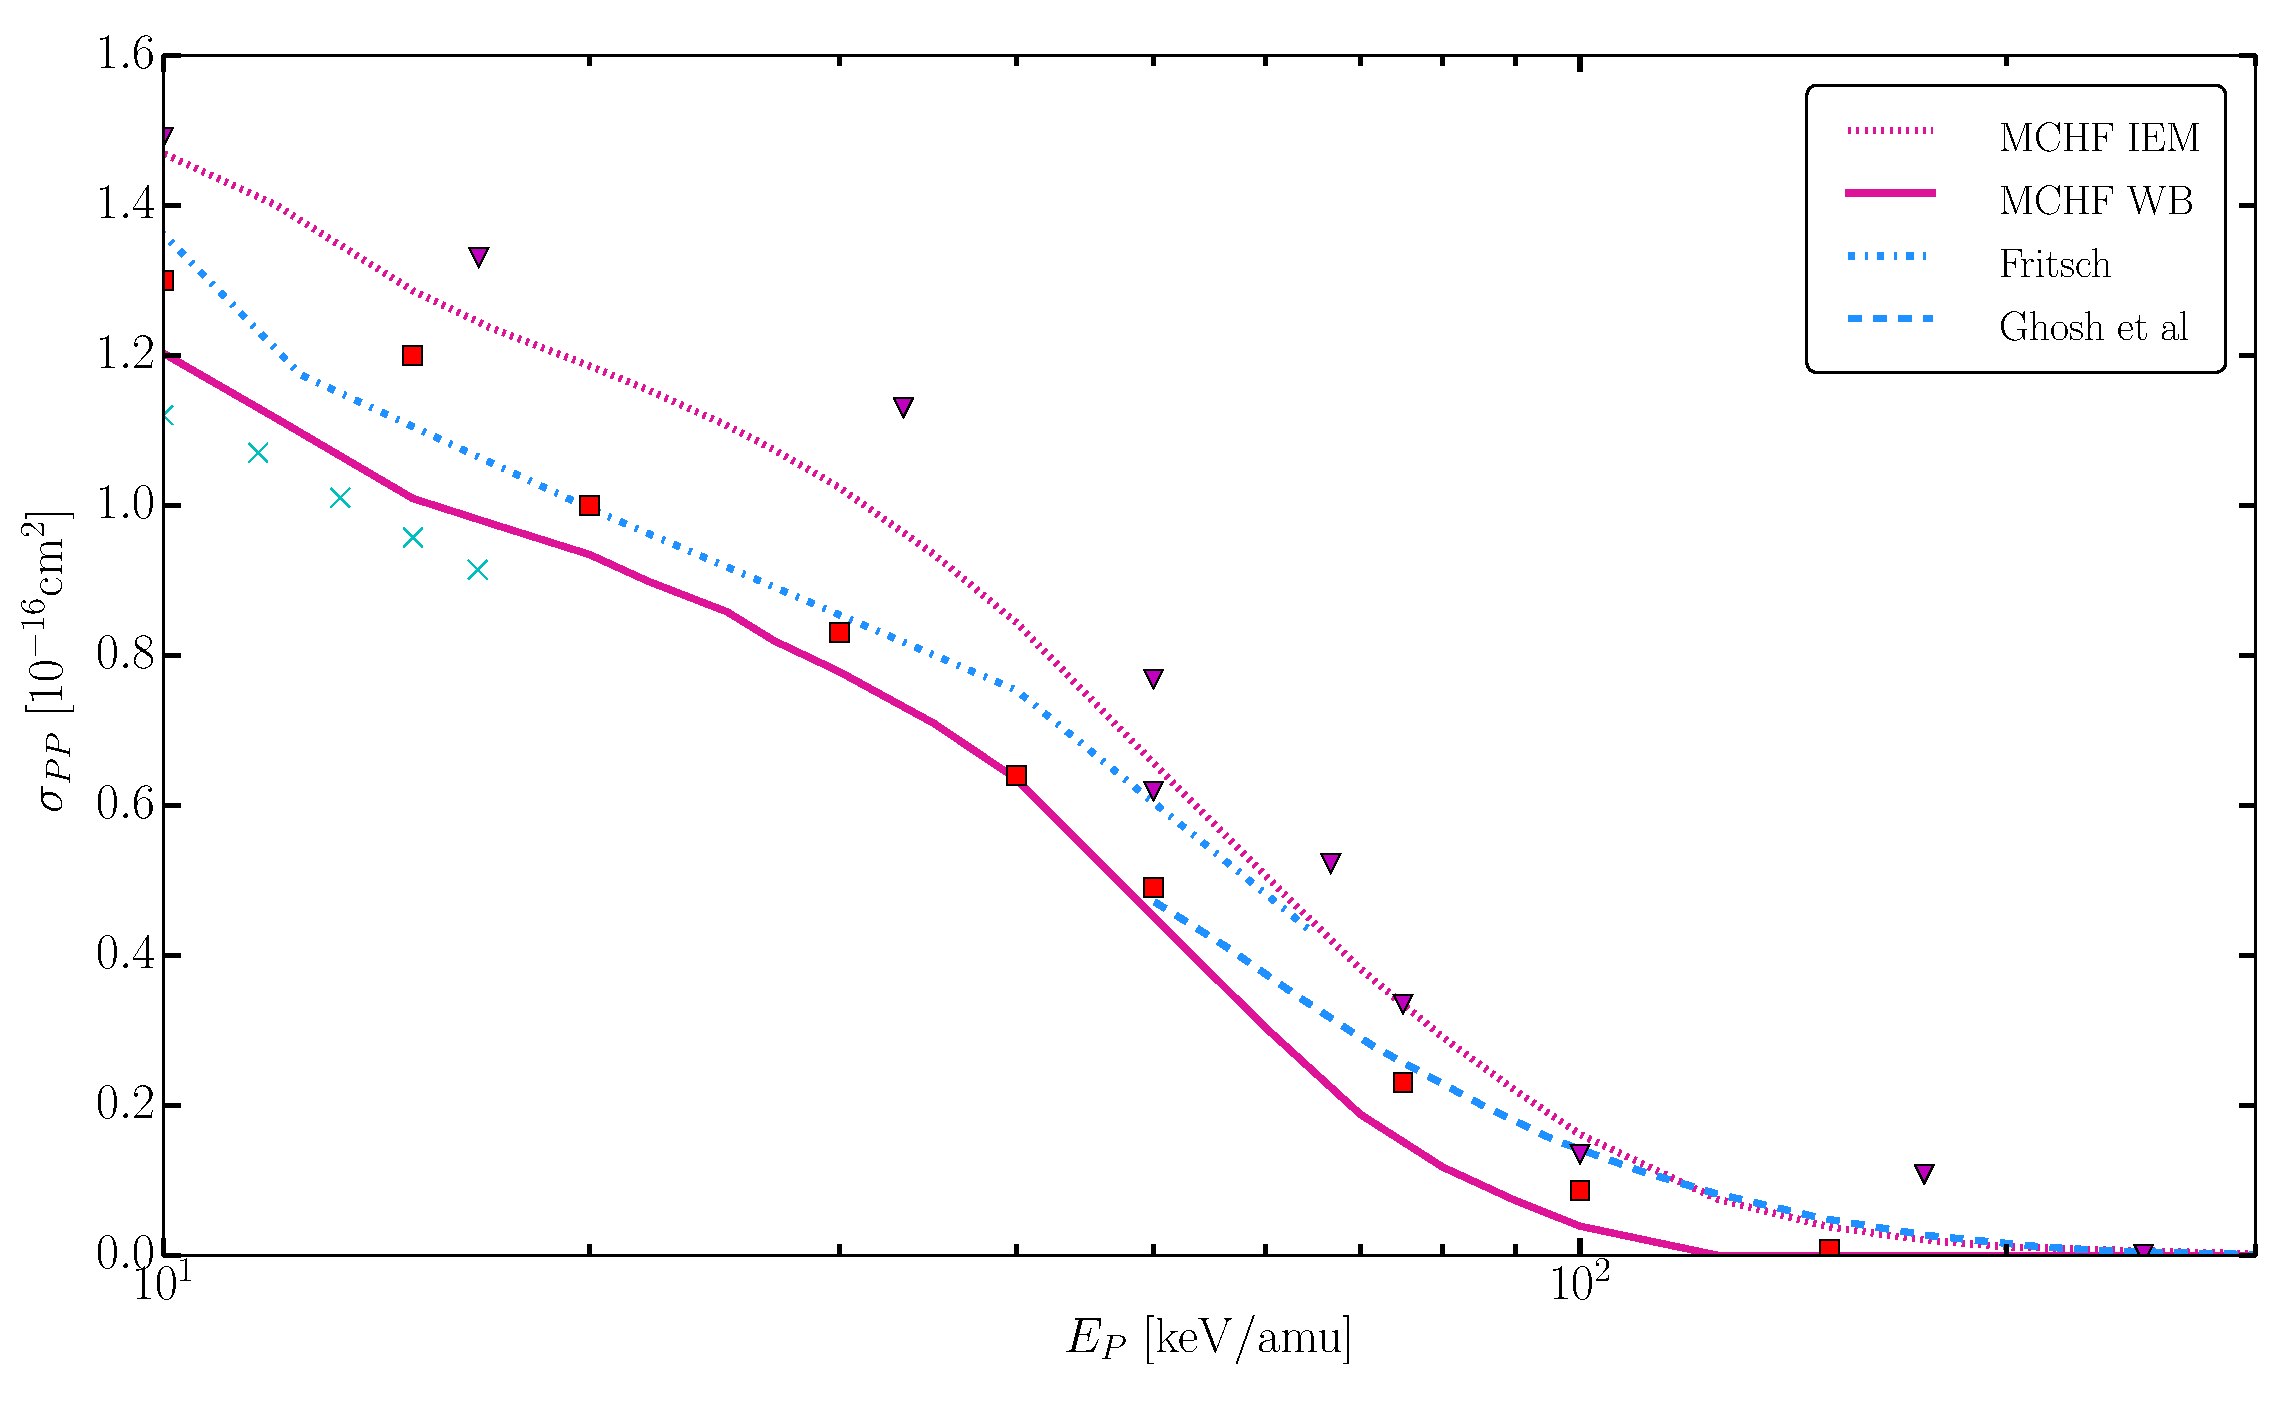
\includegraphics[width = \linewidth]{./images/he2phe/he2phe-PP.eps}
            \caption[Total cross section for double capture in He\textsuperscript{2+}-He
                     collisions.]{Total cross section for double capture in He\textsuperscript{2+}-He
                     collisions.
                     Theoretical results: Fritsch \cite{Fritsch-94} and Ghosh
                     \textit{et al}.~\cite{GDMP-08}.
                     Experimental data: {\color{RedViolet}{$\blacktriangledown$}}~\cite{Dubois87},
                     {\color{red}$\blacksquare$}~\cite{Rudd85}
                     {\color{TealBlue}$\times$}~\cite{SG74}. \label{fig:he2phe-pp}}
         \end{figure}

      \end{subsection}

   \end{section}

\end{chapter}

\begin{chapter}{\texorpdfstring{He\textsuperscript{+}}{He+}-He \label{chap:hep-he}}

\end{chapter}

\begin{chapter}{Conclusion \label{chap:con}}

   \begin{section}{\texorpdfstring{$p$}{p}-He and \texorpdfstring{He\textsuperscript{2+}}{He2+}-He
                   Collisions \label{sec:con-phe2p-he}}

   \end{section}

   \begin{section}{\texorpdfstring{He\textsuperscript{+}}{He+}-He Collisions \label{sec:con-hephe}}

   \end{section}

\end{chapter}

\begin{chapter}*{Appendices}

\end{chapter}

\cleardoublepage
\phantomsection
\addcontentsline{toc}{chapter}{References}

\bibliography{diss.bib}

\end{document}

